\documentclass{book}

% Additional packages for customization
\usepackage[utf8]{inputenc} % Encoding (use utf8 or another encoding suitable for your needs)
\usepackage[T1]{fontenc}    % Font encoding
\usepackage{lipsum}         % Example text, you can remove this in your actual document
\usepackage{fancyhdr}       % For custom headers and footers
\usepackage{listings}
\usepackage[margin=1in]{geometry}
\usepackage{xcolor}
\usepackage{hyperref}
\usepackage{graphicx}
\usepackage{tocloft}


\hypersetup{
  colorlinks=true,
  urlcolor=blue,
}

% Define page style
\pagestyle{fancy}
\fancyhf{} % Clear default header and footer

% Set the header and footer content
\fancyhead[LE,RO]{\thepage} % Page number on the left for even pages, right for odd pages
\fancyhead[RE]{\leftmark}    % Chapter title on the right for even pages
\fancyhead[LO]{\rightmark}   % Section title on the left for odd pages

% Adjust the spacing above and below the header/footer
\renewcommand{\headrulewidth}{0.5pt} % Thickness of the header rule
\setlength{\headsep}{10pt}           % Space between header and text

% Redefine the color for section entries in the table of contents
\renewcommand{\cftsecfont}{\color{blue}}

\begin{document}

\begin{titlepage}
\begin{figure}[h]
    \centering
    
\includegraphics {buet logo.jpeg}
\end{figure}
  \centering
  {\LARGE Bangladesh University of Engineering and Technology \par}
  
  \vspace{3cm}
  {\large Project Report on\par}
  {\fontsize{24pt}{28pt}\bfseries The Hive: Incident Response Platform \par}
  \vspace{2cm}
  {\large Prepared By\par}
  {\LARGE \textbf{Mohaiminul Islam - 1905018} \par}
  {\LARGE \textbf{Tanveer Rahman - 1905025} \par}
  \vspace{4cm}
  {\LARGE Department of CSE, BUET \par}
  \vfill
\end{titlepage}


\tableofcontents

\chapter{Why TheHive ?}
\section{Overview}
The Hive is a free and open-source Security Incident Response Platform (SIRS) developed by StrangeBee. It is designed to make life easier for SOCs, CSIRTs, CERTs, and any information security practitioner dealing with security incidents that need to be investigated and acted upon swiftly. The Hive is a web-based application that can be deployed on a single server or as a cluster. It relies on Apache Cassandra for data storage and Elasticsearch for indexing. A file storage solution is also required.

\subsection{Overview of Features}

The Hive provides a variety of features to help with incident response, including:

\begin{itemize}
  \item \textbf{Alert Management:} The Hive can ingest alerts from a variety of sources, such as SIEMs, firewalls, and IDS/IPS systems. It provides a dedicated and detailed alert page where users can view the alert details, make comments, and identify similar alerts.

  \item \textbf{Case Management:} The Hive allows users to create cases and associate them with alerts, tasks, and observables. Users can also define custom statuses and fields for cases.

  \item \textbf{Task Management:} The Hive allows users to create tasks and assign them to users. Users can also track the progress of tasks and set due dates.

  \item \textbf{Observable Management:} The Hive allows users to store and manage a variety of observables, such as IP addresses, domains, and hashes. Users can also define custom observable types.

  \item \textbf{User Management:} The Hive allows users to create and manage user accounts. Users can also define user permissions.

  \item \textbf{Integration Capabilities:} The Hive supports a wide range of integrations with external security tools and services. This includes integrations with SIEM systems, threat intelligence feeds, and various data enrichment sources.

  \item \textbf{Observables and Analyzers:} The platform provides the ability to analyze observables (e.g., IP addresses, domains, hashes) through the use of analyzers. Analyzers query external services or databases to gather additional information about observables, aiding in incident investigation.

  \item \textbf{Reporting:} The Hive provides a variety of reports to help organizations track their incident response activities. This aids in assessing incident response effectiveness.
\end{itemize}

\chapter{Architecture}
\section{Organization of Servers}
Each layer, TheHive application, the Database and  index engine, and file storage, is independant and can be set up as a standalone node or cluster. As a result, TheHive could be setup and work in a complex clustered archicteture, using virtual IP addresses and load balencers.
For a \textbf{standalone server}, all applications are installed on the same server.
\begin{itemize}
    \item Cassandra
    \item Elasticsearch
    \item Files are store on the filesystem (or MinIO if desired)
    \item NGINX (optional): to manage HTTPS communications
    \item TheHive
\end{itemize}
\begin{figure}[h]
    \centering
    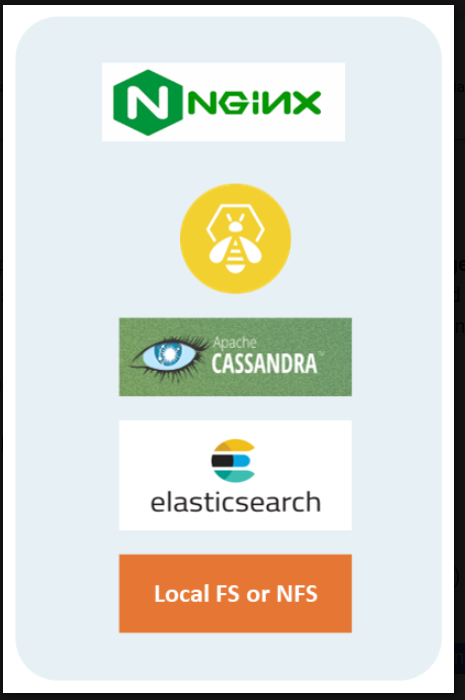
\includegraphics[scale=0.35]{Introductory Images/standalone server.png}
    \caption{Standalone server}
    \label{fig:standaloneserver}
\end{figure}

\newpage
For \textbf{Hybrid architecture} we take a different approach. TheHive and all applications of the stack are flexible enough to choose the right setup according with the needs.
\begin{figure}[h]
    \centering
    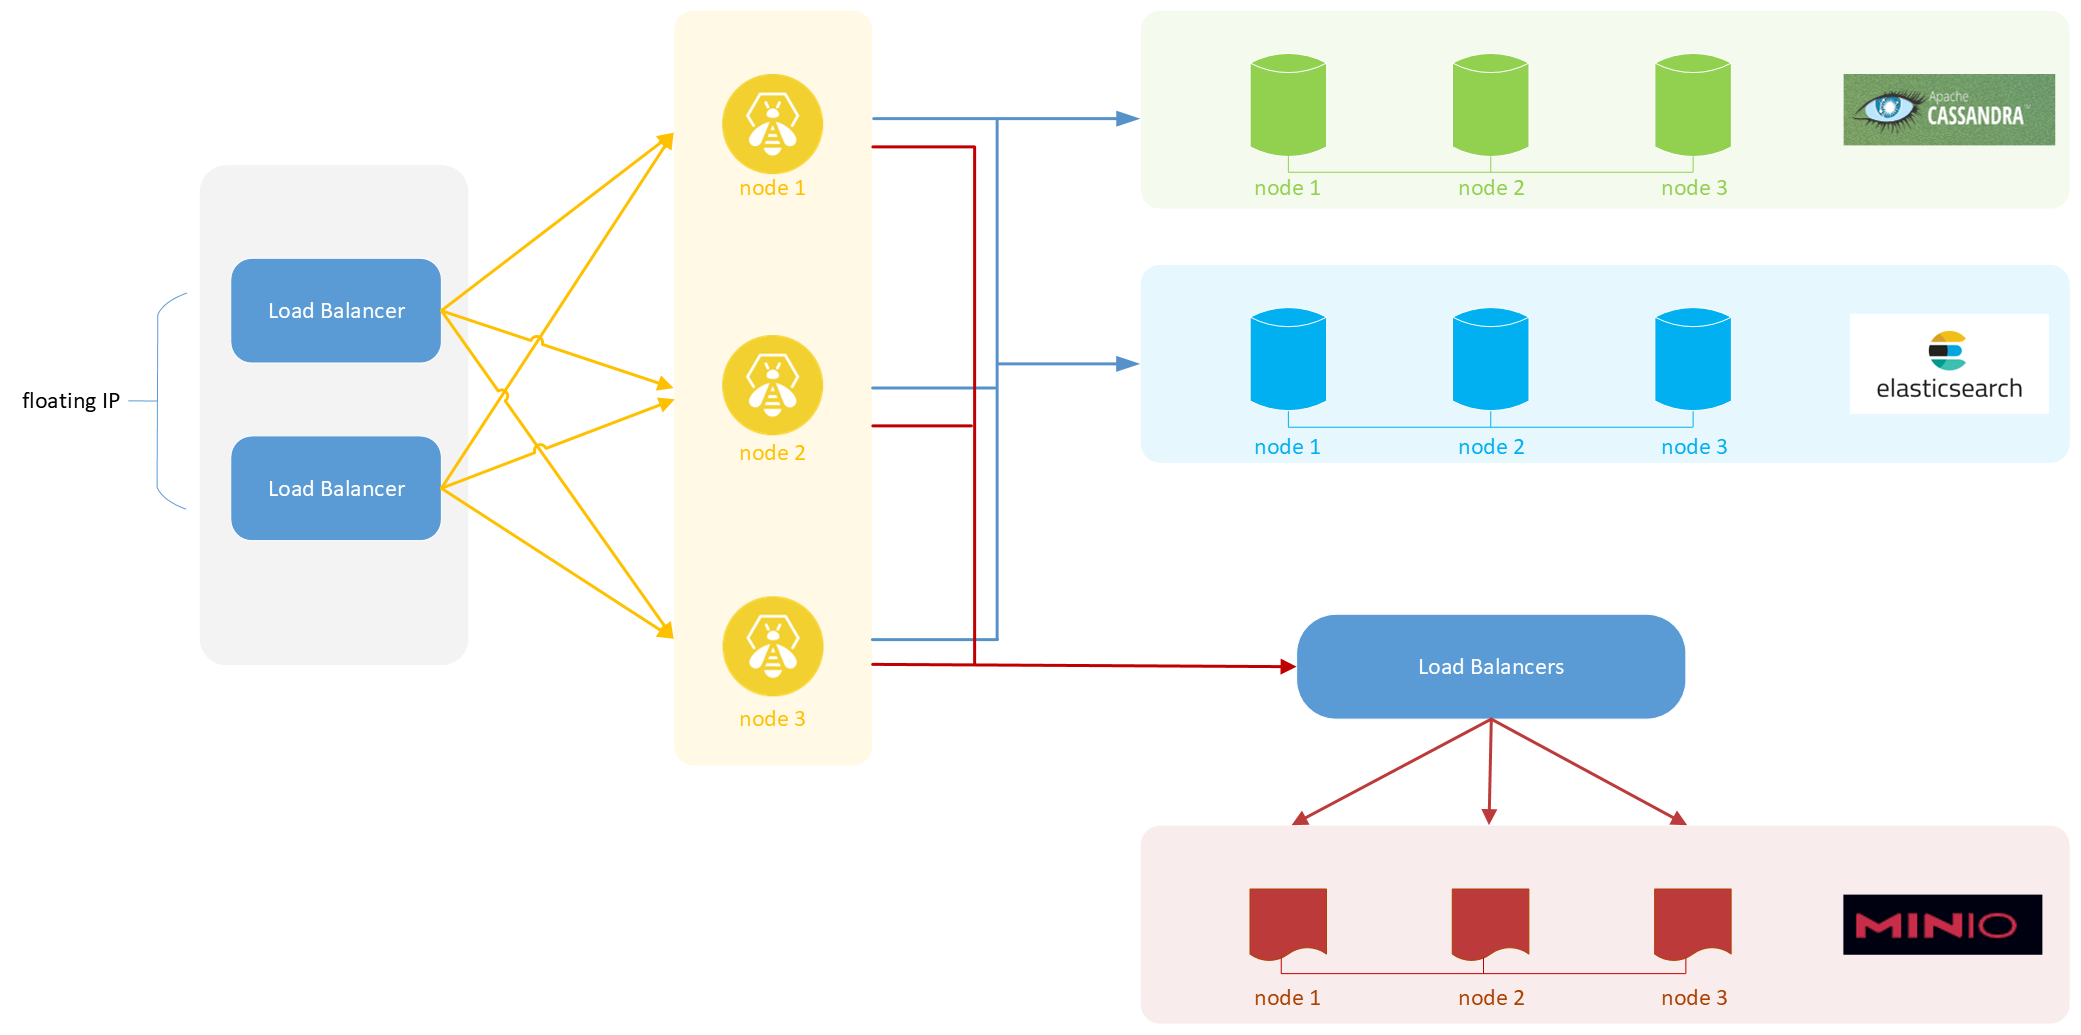
\includegraphics[scale=.5]{Introductory Images/cluster server.png}
    \caption{Hybrid Architecture}
    \label{fig:hybridarc}
\end{figure}

\newpage

\section{Overall Structure}
TheHive is written in \textit{Scala} and uses \textit{ElasticSearch} to store and access data on the back end. The front end uses \textit{AngularJS} and \textit{Bootstrap}. A number of REST API endpoints are also provided to allow for integrations and bulk actions.
\newline
\begin{figure}[h]
    \centering
    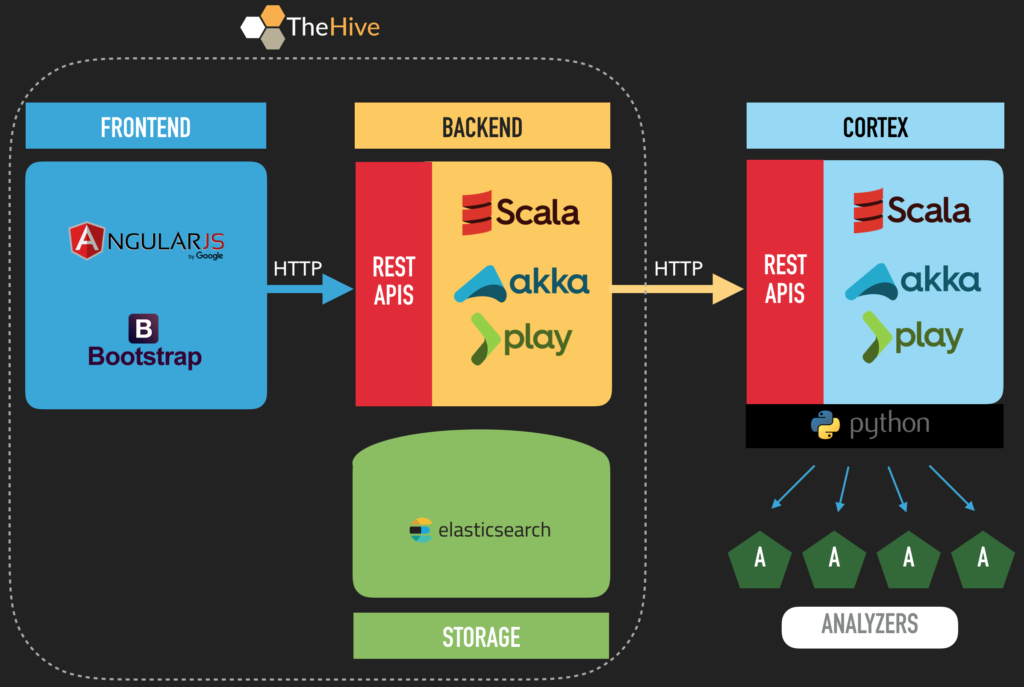
\includegraphics[scale=0.7]{Introductory Images/hive_arch-1024x687.png}
    \caption{TheHive Architecture}
    \label{fig:overallarch}
\end{figure}

\bigskip 
\bigskip

\begin{itemize}
    \item \textbf{Frontend} : The frontend is responsible for displaying the content of the system to the user. It is built using AngularJS and Bootstrap.
    \item \textbf{Backend}: The backend is responsible for processing the data and providing the data to the frontend. It is built using Scala, Akka, Play Framework, and Slick.
    \item \textbf{Cortex}: Cortex is a real-time streaming analytics platform used to process data from the backend. It is built using Scala, Akka, Play Framework, and Python.
    \item \textbf{Storage}: The storage layer is used to store the data from the system. It is made up of a distributed database, such as Elasticsearch.
    \item \textbf{Analyzers}: Analyzers are used to analyze the data from the system. They can perform tasks such as anomaly detection, fraud detection, and trend analysis.
\end{itemize}

\newpage
\subsection{Incident Response with TheHive}
\begin{figure}[h]
    \centering
    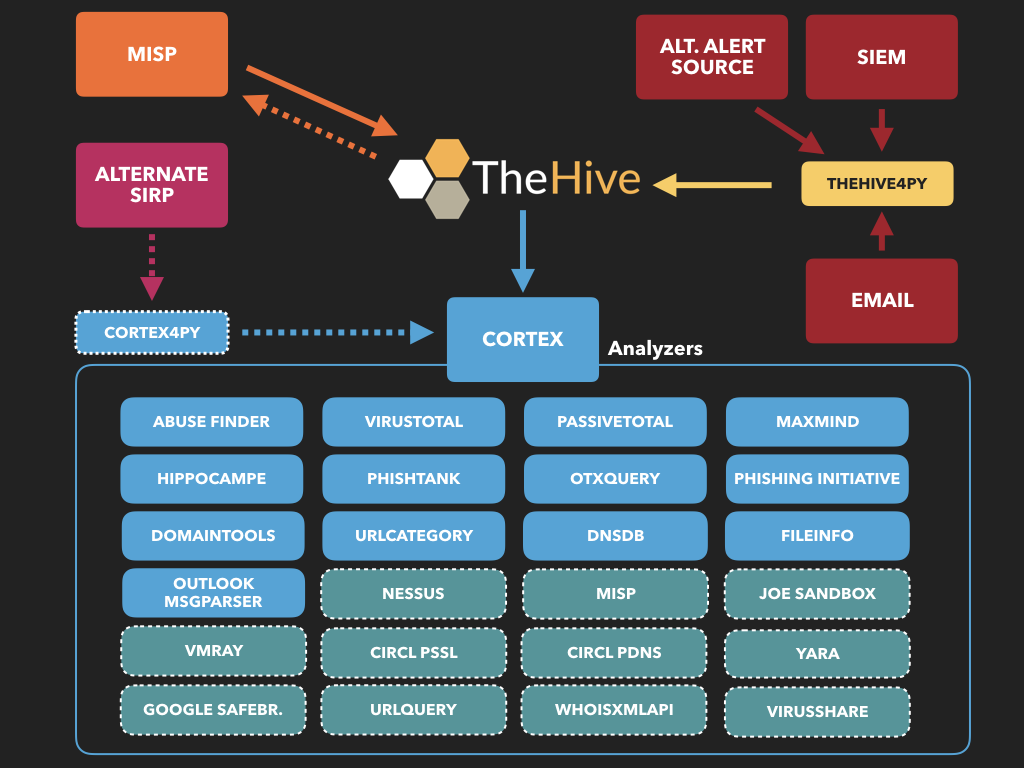
\includegraphics[scale=0.5]{Introductory Images/hive and others integration.png}
    \caption{TheHive with Cortex and MISP}
    \label{fig:hivecortexmisp}
\end{figure}




\chapter{Workflow}
\bigskip
\bigskip
\begin{figure}[h]
    \centering
    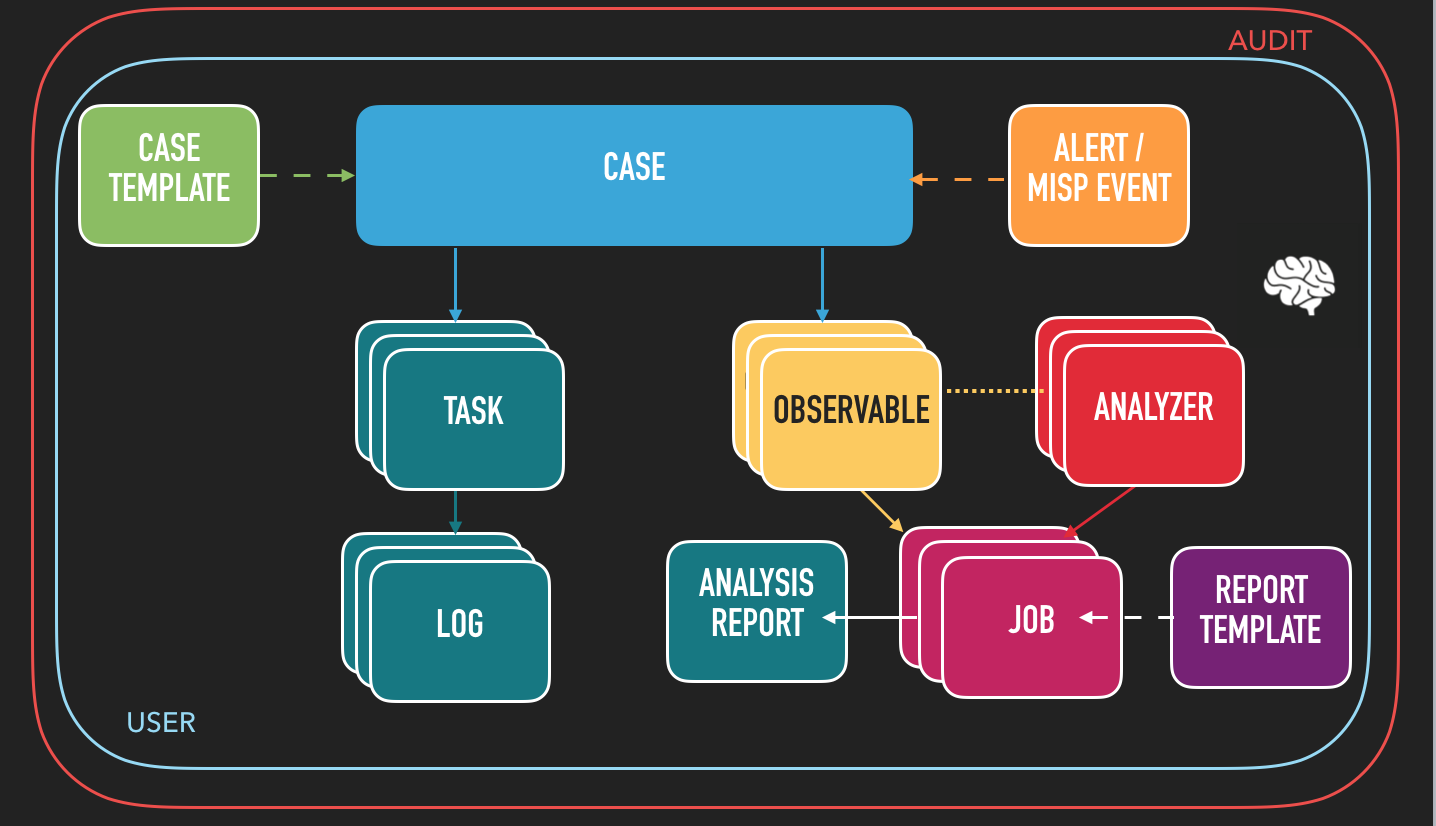
\includegraphics[scale=0.6]{Introductory Images/workflow.png}
    \caption{TheHive workflow}
    \label{fig:hiveworkflow}
\end{figure}
The Hive workflow consists of the following steps:
\begin{itemize}
    \item \textbf{Create a case:} This step is used to create a new case in the case management system. The
case should be given a unique identifier and a name that describes the incident.
    \item \textbf{Assign the case to an analyst:} This step is used to assign the case to an analyst who will
be responsible for investigating the incident. The analyst should have the appropriate skills and
experience to investigate the incident.
    \item\textbf{ Gather evidence:} This step is used to gather evidence related to the incident. The evidence can
include logs, network traffic, and screenshots. The evidence should be collected in a systematic
way so that it can be easily analyzed.
    \item \textbf{Analyze the evidence:} This step is used to analyze the evidence to identify the threat actor
and their methods. The analyst should use a variety of tools and techniques to analyze the
evidence.
    \item \textbf{Respond to the incident:} This step is used to respond to the incident, such as by isolating
the affected systems or removing the threat from the environment. The response should be
proportionate to the severity of the incident.
    \item \textbf{Close the case:} This step is used to close the case once the incident has been resolved. The
case should be closed in the case management system and the evidence should be archived.
\end{itemize}




\chapter{Installation}
We have used docker to install the hive and other related applications like Cortex and MISP. The provided installation is valid for Ubuntu or debian based operating systems. 

\section{Install Docker}

\begin{itemize}
    \item Ensure that your system has the latest information about available software packages
        \begin{verbatim}
            sudo apt-get update
        \end{verbatim}
    
    \item Installs necessary packages for securely downloading and installing software from HTTPS sources. 
        \begin{verbatim}
    sudo apt install apt-transport-https ca-certificates curl gnupg lsb-release
        \end{verbatim}

    \item Install a package containing common utilities for adding and managing software repositories.
        \begin{verbatim}
            sudo apt install software-properties-common
        \end{verbatim}
    
    \item Create the directory \textit{/etc/apt/keyrings} if it does not exist
        \begin{verbatim}
            sudo mkdir -p /etc/apt/keyrings
        \end{verbatim}
    
    \newpage
    
    \item To see the contents of the \textit{/etc/apt/keyrings} directory.
        \begin{verbatim}
            ll /etc/apt/keyrings/
        \end{verbatim}

    \item Download the Docker GPG key and saves it as \textit{/etc/apt/keyrings/docker.gpg}.
       \begin{verbatim}
    curl -fsSL https://download.docker.com/linux/ubuntu/gpg | \
    sudo gpg --dearmor -o /etc/apt/keyrings/docker.gpg
        \end{verbatim}

    \item Add the Docker repository information to the docker.list file in \newline
    \textit{/etc/apt/sources.list.d/}
        \begin{verbatim}
    echo "deb [arch=$(dpkg --print-architecture) signed-by=/etc/apt/keyrings/docker.gpg] \
    https://download.docker.com/linux/ubuntu $(lsb_release -cs) stable" | \
    sudo tee /etc/apt/sources.list.d/docker.list > /dev/null
        \end{verbatim}

    \item Updates the package lists to include the Docker repository.

        \begin{verbatim}
            sudo apt update
        \end{verbatim}
    
    \item Install Docker and related packages.
        \begin{verbatim}
        sudo apt-get install docker-ce docker-ce-cli containerd.io docker-compose-plugin
        \end{verbatim}
\end{itemize}


\section{Create Docker Container}
Docker Installation is Done. For checking the Docker Info: 
    \begin{verbatim}
        sudo docker info
    \end{verbatim}
To create new Docker Container :
    \begin{verbatim}
        sudo docker run hello-world
    \end{verbatim}

\section{Install The Hive}
\begin{itemize}
    \item Create a new directory named 'TheHive' in the current working directory.
    \begin{verbatim}
        mkdir ‘TheHive’
    \end{verbatim}
     
     \item Go to the directory
    \begin{verbatim}
        cd ‘TheHive’
    \end{verbatim}

    \item Creates an empty file named 'docker-compose.yaml' in the current working directory.
    \begin{verbatim}
        touch docker-compose.yaml
    \end{verbatim}

    \newpage

    \item Copy contents from the provided link to the .yaml file.
        \href{https://github.com/ls111-cybersec/thehive-cortex-misp-docker-compose-lab11update/blob/main/docker-compose.yml}{GitHub Link}
    \item If your System does not have the docker-compose plugin then install it.
        \begin{itemize}
            \item To check if the plugin is available:
                \begin{verbatim}
                    docker-compose -version
                \end{verbatim}
            \item If not installed then install it
                \begin{verbatim}
                    sudo apt-get install docker-compose-plugin
                \end{verbatim}      
        \end{itemize}
    \item Execute the Docker Compose command to start the services defined in the 'docker-compose.yaml' file in detached mode (-d).
        \begin{verbatim}
            sudo docker-compose up -d
        \end{verbatim} 
\end{itemize}

After completing the installation, The Hive will be opened at \href{http://localhost:9000/}{The Hive}.

\bigskip
\bigskip
\bigskip
\bigskip

\textbf{Reference Videos:}
\begin{enumerate}
    \item \href{https://www.youtube.com/watch?v=ILdziITdSag&ab_channel=InfrontofIT}{Install Docker}
    \item \href{https://www.youtube.com/watch?v=Vr4flc55S5c&pp=ygUaaW5zdGFsbCB0aGUgaGl2ZSBpbiB1YnVudHU%3D}{The Hive installation}
\end{enumerate}



\chapter{Admin Side Management}
TheHive is a web application that can be installed on a server and accessed from a web browser. It has a web-based administration interface that allows administrators to configure the tool according to their needs.
\newline
TheHive allows administrators to create multiple organizations within the tool. Each organization can have its own set of users, roles, permissions, and notifications. This allows for better separation of duties and responsibilities between different teams within an organization, such as a SOC team and a CSIRT team.
\newline

\section{Organization Management}
\subsection{Create Organization}
\begin{figure}[h]
    \centering
    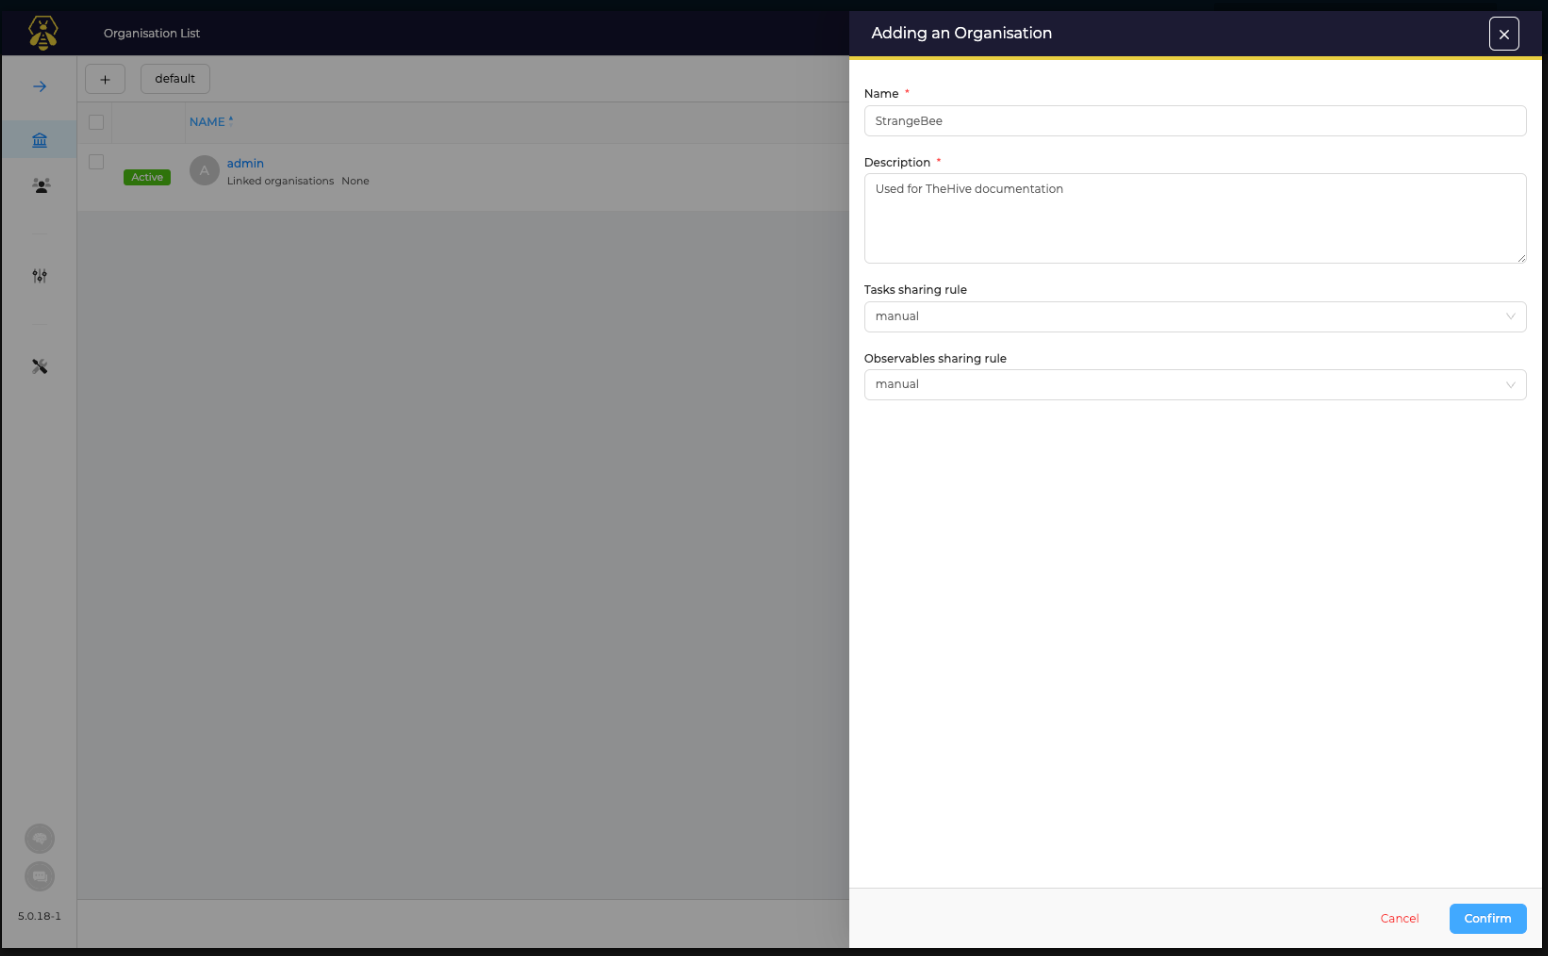
\includegraphics[width=0.7\linewidth]{Organization_images/add_org.png}
    \caption{Create Organization}
    \label{fig:createorg}
\end{figure}
To create an organization: 
\begin{itemize}
    \item Click on the + button
    \item Fill up the necessary fields
    \item Click on Confirm
\end{itemize}

\newpage

\subsection{Link Organization}
By default, organisations are not linked each other: each one does not know about the others on the instance. So, we can link organizations so that two organizations can also collaborate with each other.

In order to create Link between organizations, 
\begin{itemize}
    \item Click on the \textbf{Linked Organizations} tab in the detailed view 
    \item Click on \textbf{Manage linked Organisations}
\end{itemize}
\begin{figure}[h]
    \centering
    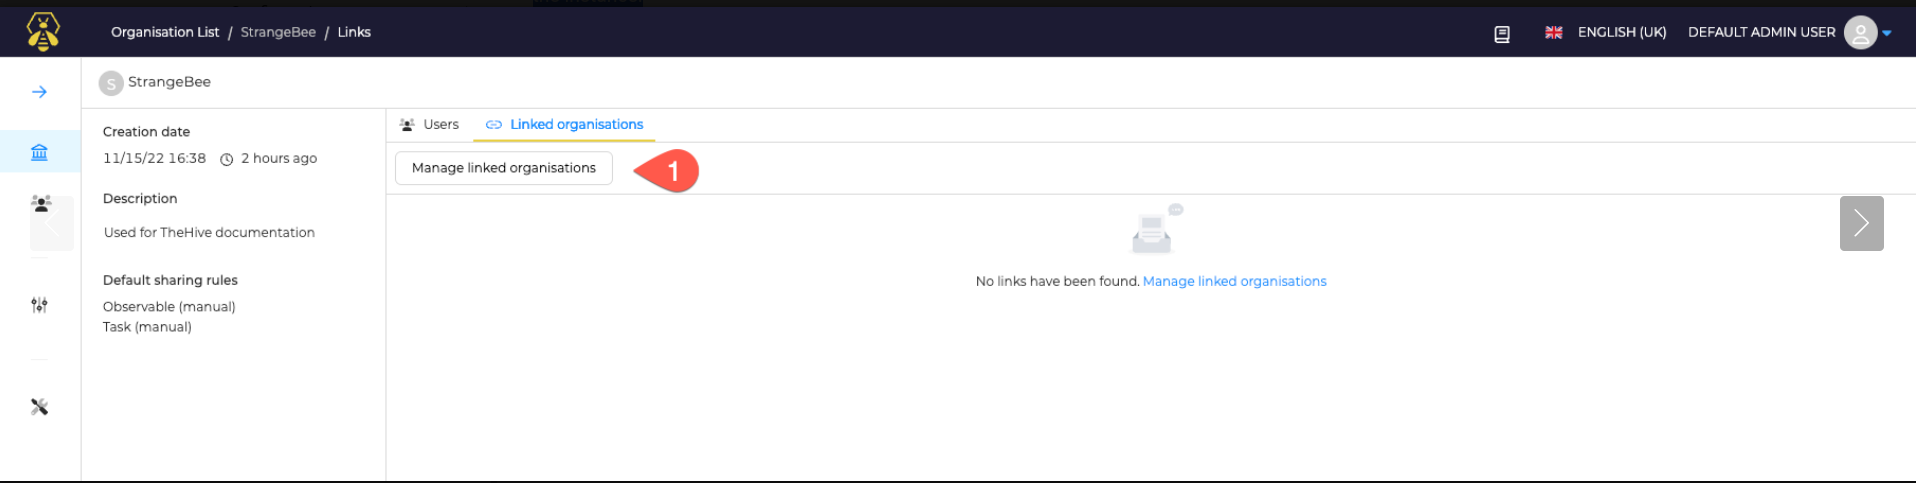
\includegraphics[width=0.8\linewidth]{Organization_images/Link_manage.png}
    \caption{Manage Linked Organizations}
    \label{fig:linkmanage1}
\end{figure}
\bigskip
Select the organizations to be linked with each other and the details page is viewed in fig {\ref{fig:linkmanage2}}. \bigskip

Three types of links are available. They are :
\begin{itemize}
    \item \textbf{Default}: Cases created by the current Organisation will not be shared with the other one
    \item \textbf{Supervised}: Cases created by the current Organisation will be automatically shared with the other one, with the profile Analyst
    \item \textbf{Notify}: Cases created by the current Organisation will be automatically shared with the other one, with the profile Read-only
\end{itemize}
\newpage
\begin{figure}[h]
    \centering
    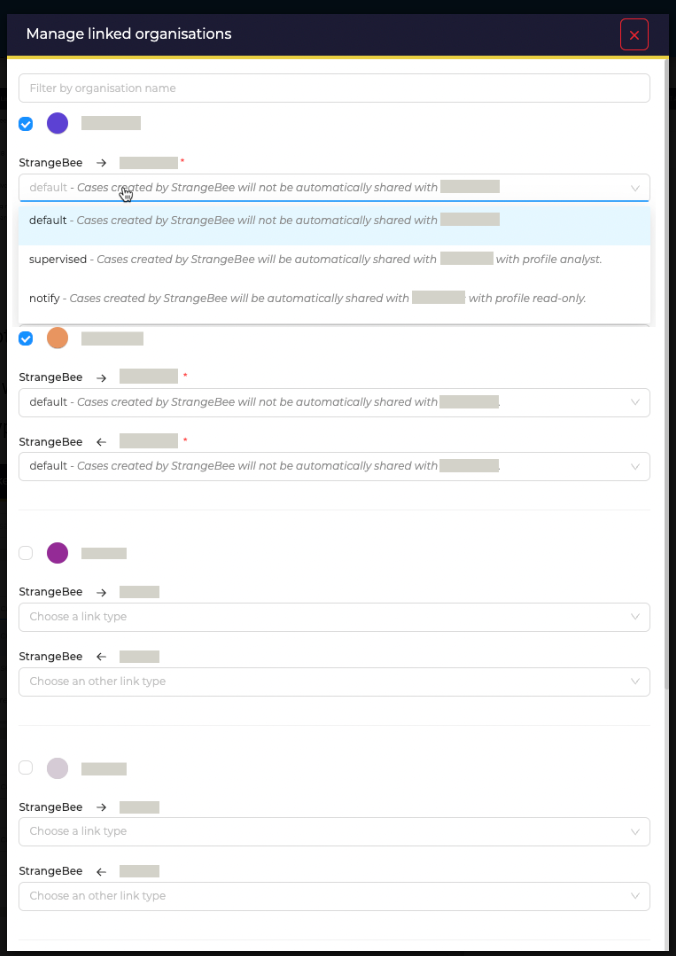
\includegraphics[width=0.7\linewidth]{Organization_images/form for link.png}
    \caption{Form for Link Management}
    \label{fig:linkmanage2}
\end{figure}

\newpage

\section{User Management}
TheHive allows administrators to create multiple user accounts within the tool. Each user account can have its own set of roles and permissions. Accounts can be created or edited from several places in TheHive:
\begin{itemize}
    \item As Administrator, in the Users view
    \item As Administrator in the detailed page of an Organisation
    \item As Org-admin, in the Organisation configuration page
    \item As Administrator of the platform, open the Users page.
\end{itemize}

\subsection{Permission and Roles}
Users are given Permissions by their roles. Permissions are defined for each entity of the application.
The following entities are available:
\begin{itemize}
    \item \textbf{Admin}: Administrators have full control over TheHive platform. They can create, modify, and delete accounts, organizations, and configurations. Administrators typically manage the overall settings and ensure the platform functions smoothly. Their privileges:
        \begin{itemize}
            \item Full access to all features and functionalities.
            \item User and organization management.
            \item Configuration and system settings control.
            \item Incident case management.
        \end{itemize}
    \item \textbf{Analyst}:Analysts are standard users responsible for working on incident cases and investigations within TheHive. They have access to case management and analysis tools to investigate and respond to security incidents. Their privileges:
        \begin{itemize}
            \item Access to incident case management
            \item Ability to work on and update cases.
            \item Collaboration with other analysts.
            \item Limited access to system configurations.
        \end{itemize}
    \item \textbf{Org-admin} (\textit{Organization Administrator}): Organization administrators have administrative privileges limited to a specific organization within TheHive. They can manage users, incidents, and configurations for their assigned organization. Their privileges:
        \begin{itemize}
            \item User management within their organization.
            \item Incident case management within their organization.
            \item Limited access to system-wide configurations
            \item May not have access to other organizations’ data.
        \end{itemize}
    \item \textbf{Read-only} Read-only users have limited access and are primarily meant for users who need to view incident cases and data without making changes or updates. They can review and gather information but cannot modify cases. Their privileges:
        \begin{itemize}
            \item View-only access to incident cases and data
            \item Cannot modify or update cases.
            \item Limited interaction with the platform
        \end{itemize}
\end{itemize}





\chapter{Case}
A case provides information on suspicious activity in the environment. Security analysts can conduct specific analysis based on cases to assess the possibilities of threats. 

\section{Create Case}
The Header has a button named \textbf{CREATE CASE +}. 
\begin{figure}[h]
    \centering
    
\includegraphics[width=0.8\linewidth]{Case_images/createcase+.png}
    \caption{Create Case +}
    \label{fig:createcasebutton}
\end{figure}

A new screen opens and from this screen we can open new cases.
\begin{figure}[h]
    \centering
    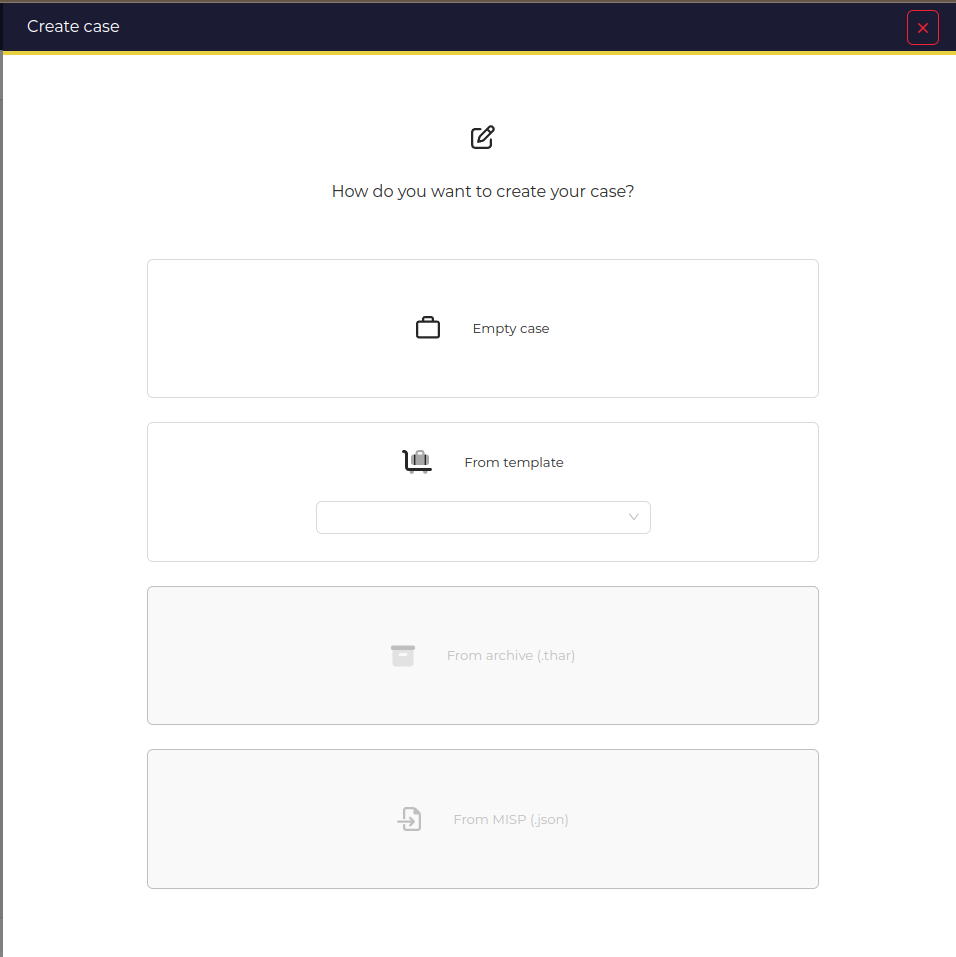
\includegraphics[width=0.5\linewidth]{Case_images/createcaseoverlay.png}
    \caption{New page for Create Case}
    \label{fig:createcaseoverlay}
\end{figure}

\newpage

\subsection{Create Empty Case}
Create a new empty case after filling up the necessary information. 
\begin{figure}[h]
    \centering
    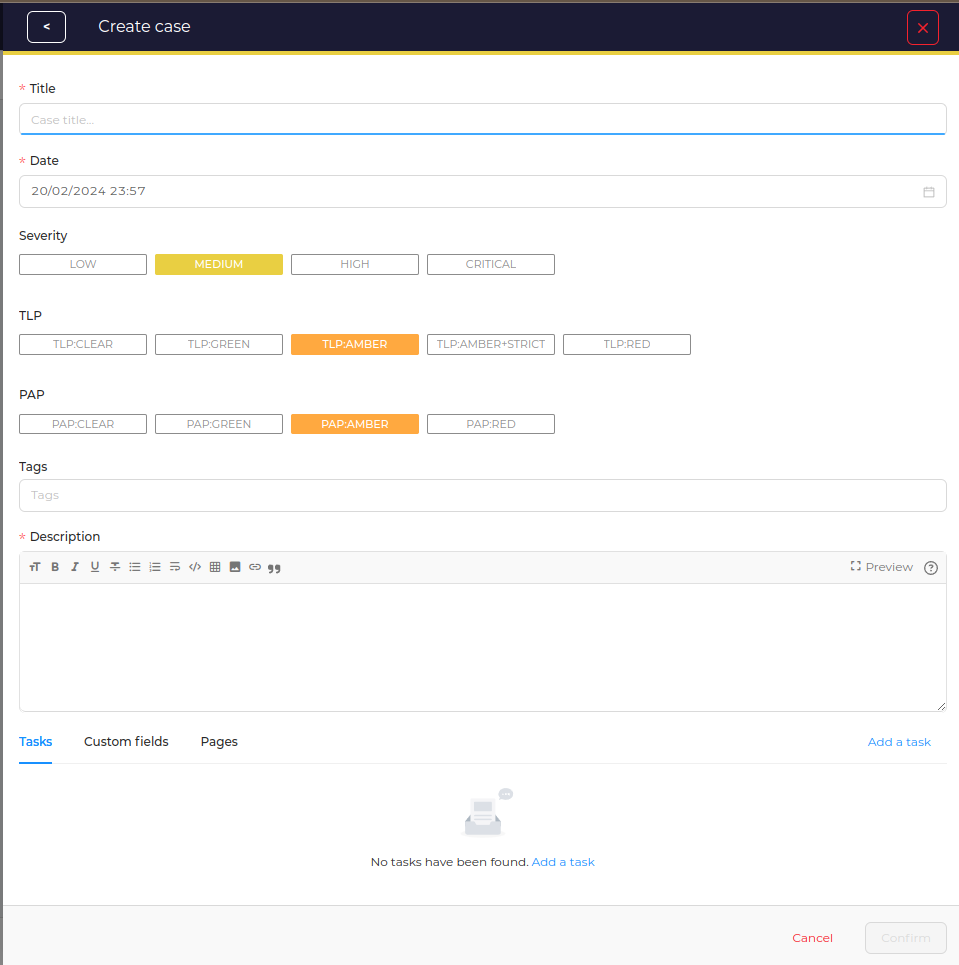
\includegraphics[width=0.9\linewidth]{Case_images/emptycase.png}
    \caption{Create empty case}
    \label{fig:emptycaseoverlay}
\end{figure}

\subsubsection{PAP(Permissible Actions Protocol)}
Defines what actions you can take with the information without alerting the attacker.
\begin{itemize}
    \item \textbf{White:} No restrictions. Any action can be taken openly.
    \item \textbf{Green:} Active actions like blocking IPs are okay. But avoid actions that might reveal your awareness of the attack, like sending honeypots.
    \item \textbf{Amber:}  Only passive actions like monitoring are allowed. Don't interact with the attacker directly.
    \item \textbf{Red:} No detectable actions. Treat the information as highly sensitive and keep all analysis hidden.
\end{itemize}

\newpage

\subsubsection{TLP (Traffic Light Protocol)}
TLP defines the confidentiality level of information within the case
\begin{itemize}
    \item \textbf{White:} Public information, freely distributable.
    \item \textbf{Green:} Internal use only, within your organization.
    \item \textbf{Amber:} Limited distribution outside your organization, with specific need-to-know basis
    \item \textbf{Red:} Classified information, restricted to a very small group with strict control. 
\end{itemize}

\subsubsection{Tasks}
\begin{itemize}
    \item Tasks are specific actions to be taken during the investigation and response process for a case.
    \item They offer a structured way to assign responsibilities, track progress, and ensure all necessary steps are completed.
\end{itemize}

\subsubsection{Custom Fields}
\begin{itemize}
    \item Custom fields extend the default information captured in a case to accommodate specific needs or workflows.
    \item These fields allow capturing additional context relevant to the incident, like affected systems, impact level, or mitigation actions taken.
    \item Custom fields enhance data collection, reporting, and filtering capabilities within TheHive.
\end{itemize}

\bigskip
\bigskip


\newpage


\subsection{Create a new case from EDR template}
We can also create a new case from builtin MISP template where few tasks, observables and some
other routines already added to make things easy.
\bigskip
\begin{figure}[h]
    \centering
    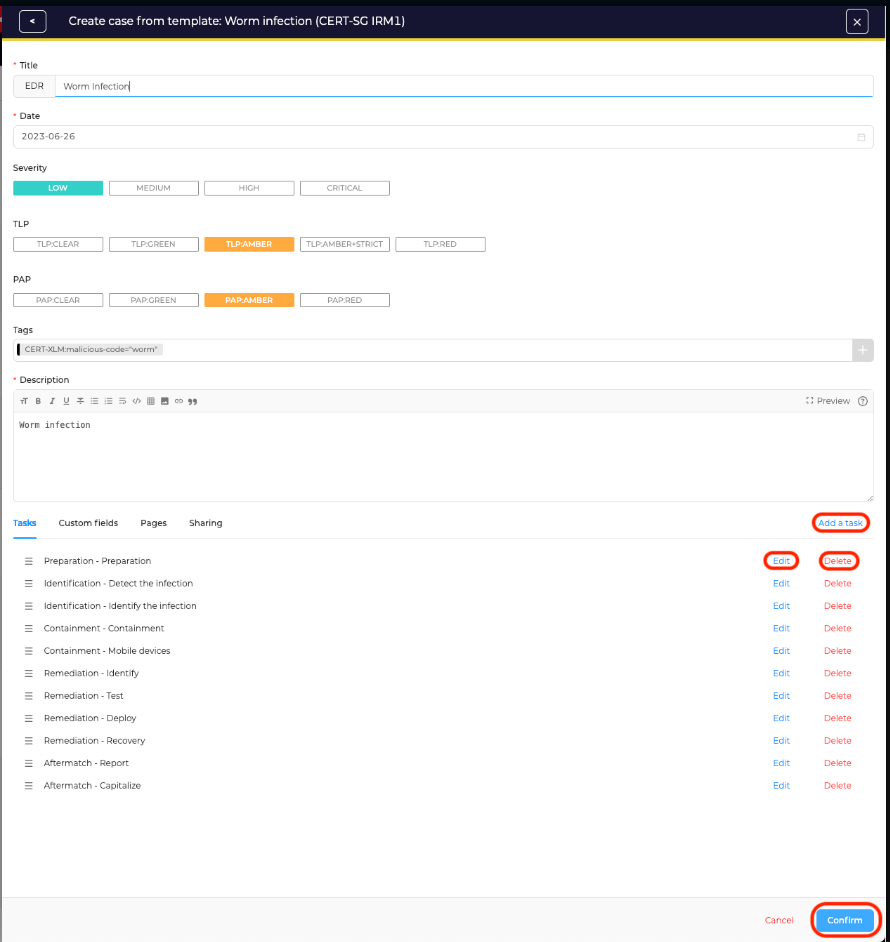
\includegraphics[width=.8\linewidth]{Case_images/casefromedr.png}
    \caption{Case from EDR Template}
    \label{fig:casefromedr}
\end{figure}

\newpage
\subsection{Create a new case from Phishing template}
Phishing templates let the analyst think in a attacker’s way. So, creation of such cases from attacker’s
perspective sometimes give analysts a great advantage in analysis and study.
\bigskip
\begin{figure}[h]
    \centering
    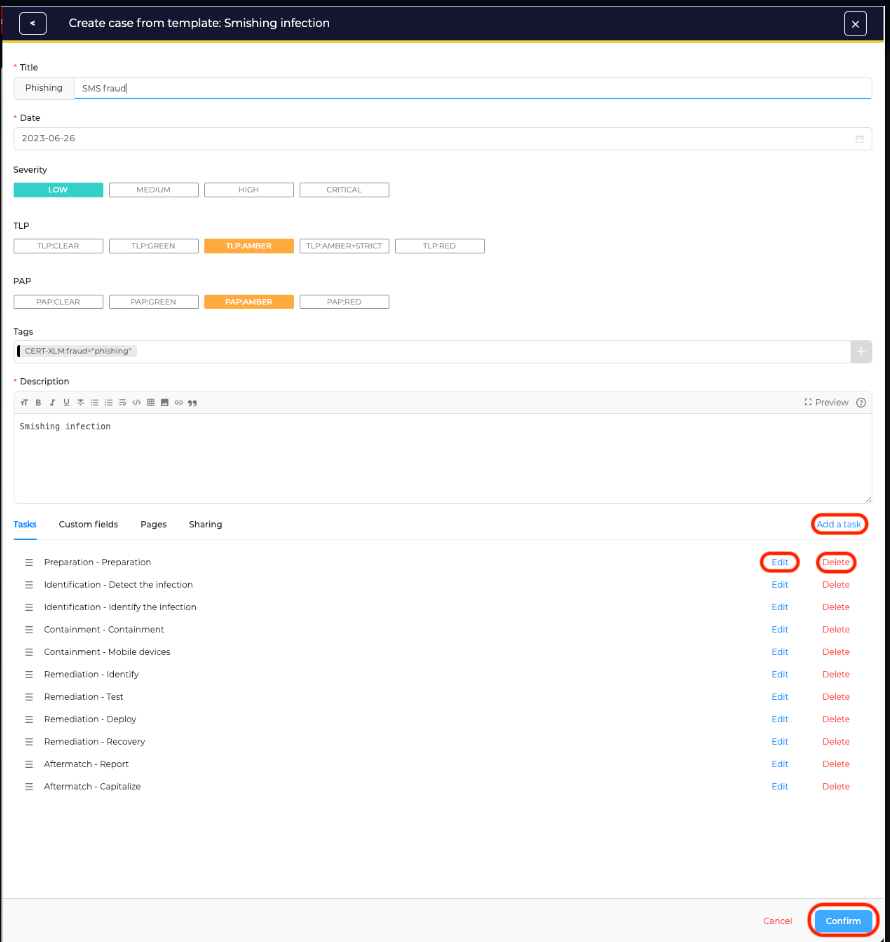
\includegraphics[width=.8\linewidth]{Case_images/casefromphishingtemplate.png}
    \caption{Case from Phishing Template}
    \label{fig:casefromphishingtemplate}
\end{figure}

\newpage

\subsection{Create a new case from MISP}
Files exported from MISP can be used to create new Case in Hive. The MISP file exported as .json and then uploaded to create a new case
\bigskip
\begin{figure}[h]
    \centering
    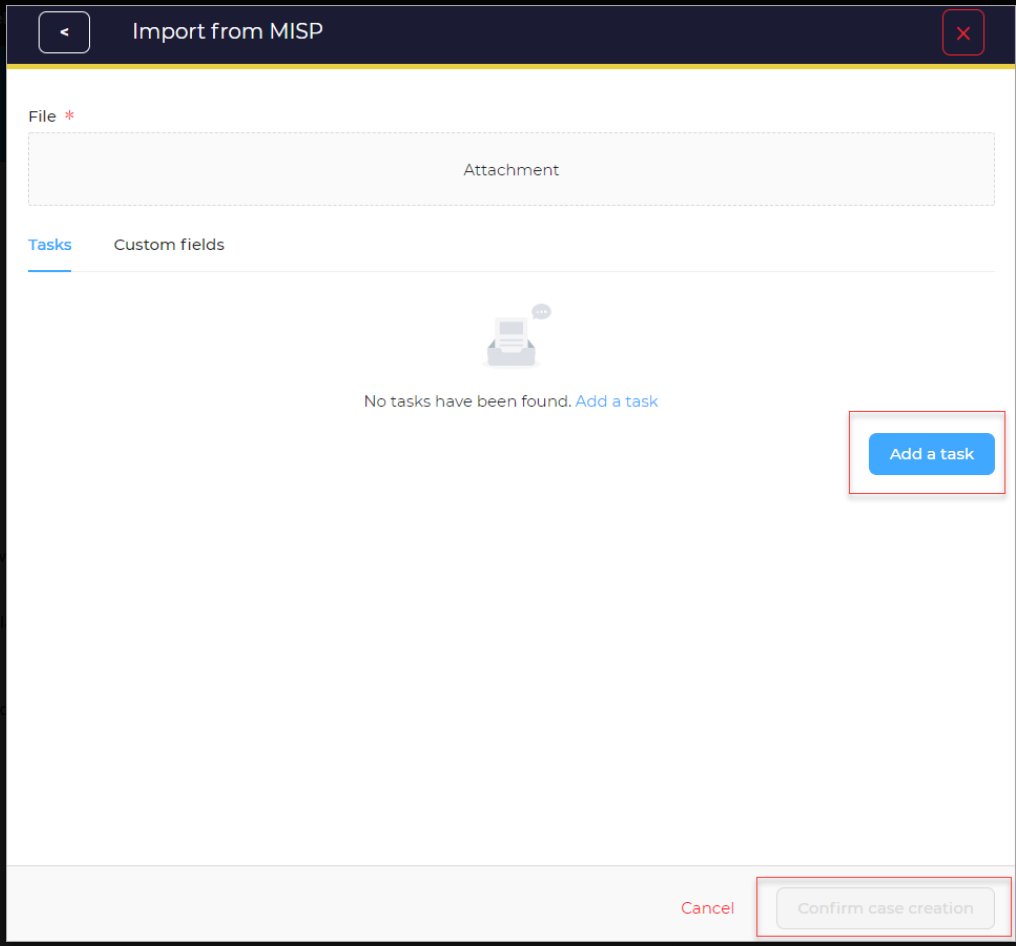
\includegraphics[width=.8\linewidth]{Case_images/MISP.png}
    \caption{Case from MISP}
    \label{fig:casefromMISP}
\end{figure}

\newpage

\section{Case Properties}
\subsection{Tasks}
The task feature in TheHive is a crucial component for managing the investigation process within a case. It allows the user to break down the investigation into smaller, actionable steps, ensuring a structured and efficient approach.
\bigskip

\textbf{Why Task ?}
\begin{itemize}
    \item Structured Approach
    \item Improved Collaboration
    \item Accountability
    \item Improved Communication
\end{itemize}
\bigskip

The tasks are defined by the organization manager. They are grouped together for better Communication and collaboration. 
\newline
\newline
The organization manager can assign certain task to a certain analyst and can give a deadline for the completion of the task. Thus, proper accountability is maintained.
\newline
\newline
 Tasks can be prioritized based on their urgency and importance to the overall investigation. 
\newline
\newline
Each task can have its own dedicated comment section. This enables analysts to discuss the task, share findings, and collaborate effectively. Analysts can document their actions and findings related to the task by adding logs. 

\bigskip
\begin{figure}[h]
    \centering
    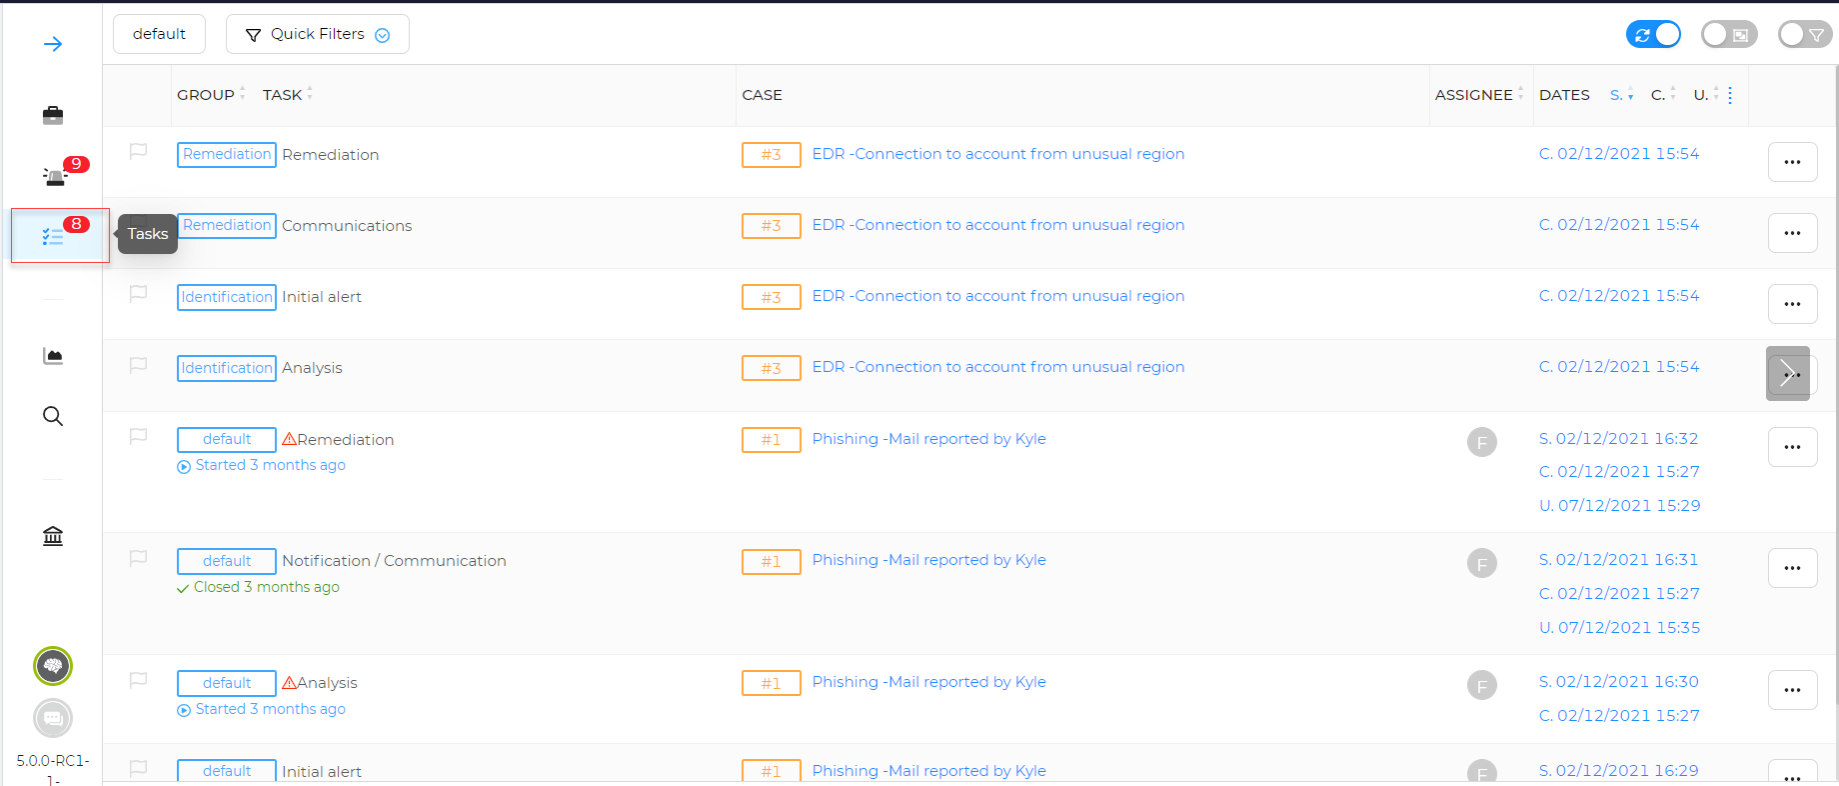
\includegraphics[width=.8\linewidth]{Case_images/Task1.png}
    \caption{Task Page}
    \label{fig:task1}
\end{figure}


\newpage


\subsection{Observables}
Observables represent stateful properties   or measurable events that are pertinent to the operation of computers and networks. The IP of the Source, the Destination IP, the PCAP files all can be added as observables. 

\begin{figure}[h]
    \centering
    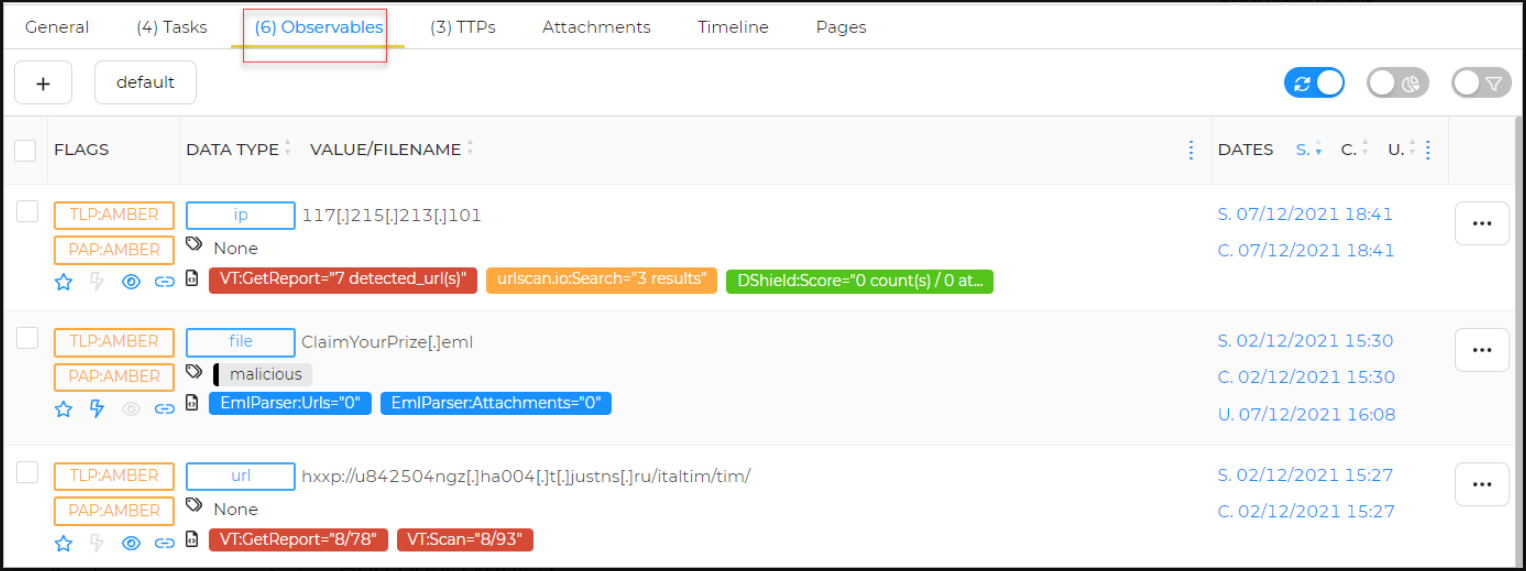
\includegraphics[width=.8\linewidth]{Case_images/observables.png}
    \caption{Observables }
    \label{fig:observables}
\end{figure}

The create observables has the PAP, TLP, fields like before. It also has some special fields. Like:
\begin{itemize}
    \item \textbf{Is IOC} This is a button, that can be truned on or off. IOC means \textit{Indicator of Compromise}. This allows the users to centralize evidence and track potential malicious activity effectively.
    \item \textbf{Ignore Similarity} This is also a button. Which determines whether we want to co-relate this ovservable with other existing observables.
    \item \textbf{Has Been Sighted} Button that serves the purpose of checking if the observable has already sighted in the system or if it has assigned before. 
\end{itemize}
\bigskip
\bigskip
We can perform various actions over the observables, like:
\begin{itemize}
    \item Delete
    \item Run Analyzers
    \item Export - To download the observable 
    \item Copy 
\end{itemize}

\newpage

\subsection{TTP}
\textbf{TTP} stands for \textit{Tactics, Techniques, and Procedures}. These represent the specific methods attackers employ to carry out their malicious activities.

\begin{enumerate}
    \item \textbf{Tactics} Broad approaches or goals attackers aim to achieve during an attack (e.g., initial access, persistence, privilege escalation, data ex-filtration).

    \item \textbf{Techniques} Specific tools and methods attackers use to implement their tactics (e.g., phishing emails, exploiting vulnerabilities, installing malware).

    \item \textbf{Procedures} Step-by-step instructions that detail how attackers execute their techniques (e.g., crafting a social engineering email, deploying a specific exploit kit).
\end{enumerate}
\bigskip
\bigskip
\begin{figure}[h]
    \centering
    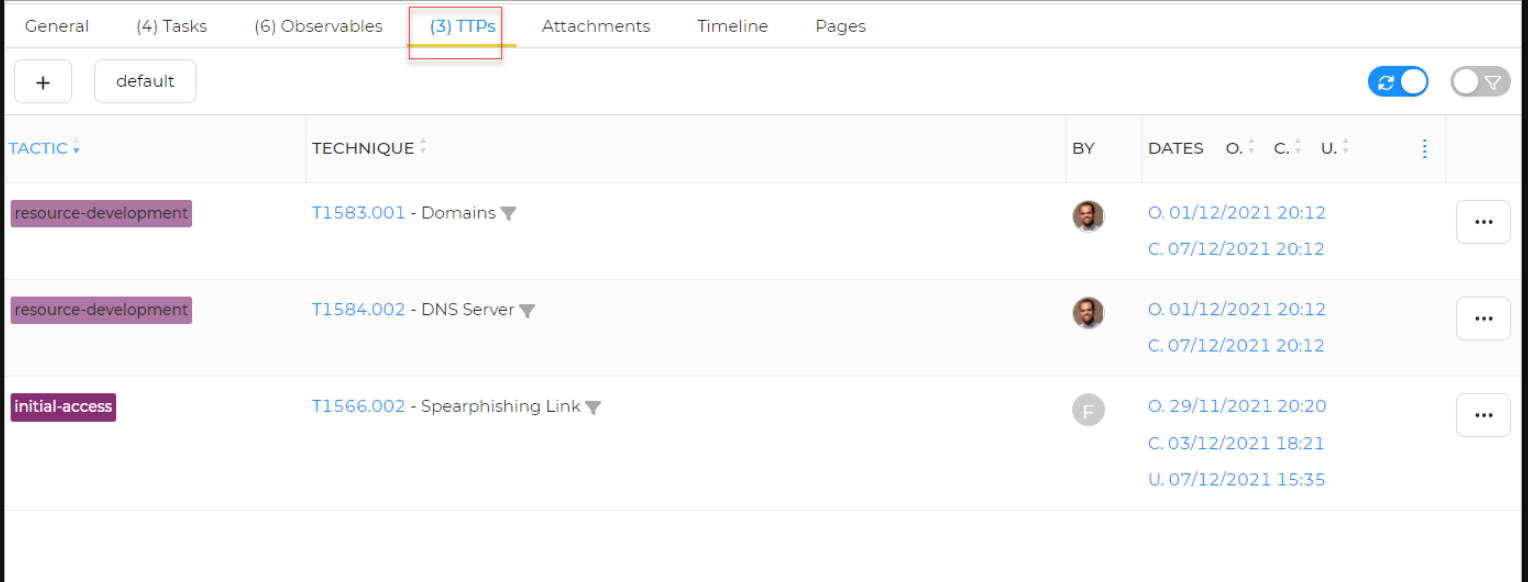
\includegraphics[width=.8\linewidth]{Case_images/TTP.png}
    \caption{TTP}
    \label{fig:ttp}
\end{figure}
\bigskip
\bigskip
The use of TTP :
\begin{enumerate}
    \item Improves Threat Detection
    \item More Effective Response
    \item Proactive Mitigation - By studying TTPs, security teams can develop preventive measures to thwart attacks that rely on those methods. 
\end{enumerate}

\newpage
\subsection{Add Tags}
\begin{itemize}
    \item Choose tags from the Taxonomy. The selected tag will appear in the Selected Tags box
    \item Click the Add selected tags button.
\end{itemize}
\begin{figure}[h]
    \centering
    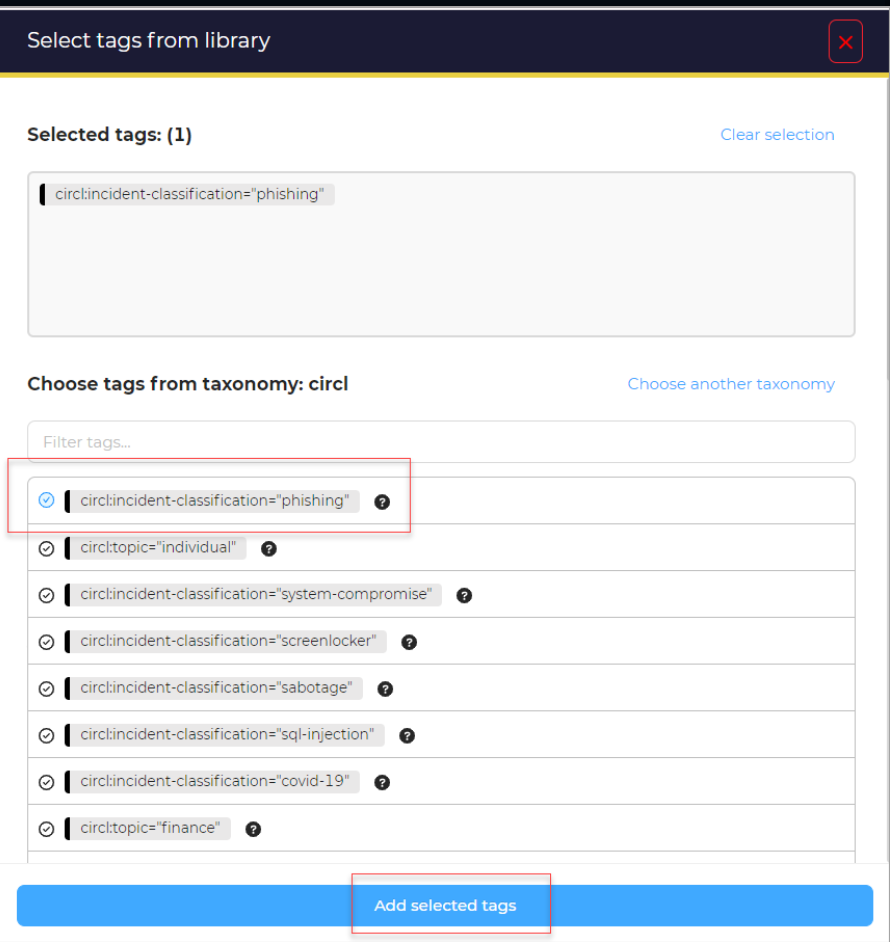
\includegraphics[width=.8\linewidth]{Case_images/addTags.png}
    \caption{add Tags}
    \label{fig:addtags}
\end{figure}

\newpage

\section{Demonstration of a Case Creation}
\subsection{Organization and Users}
\begin{figure}[h]
    \centering
    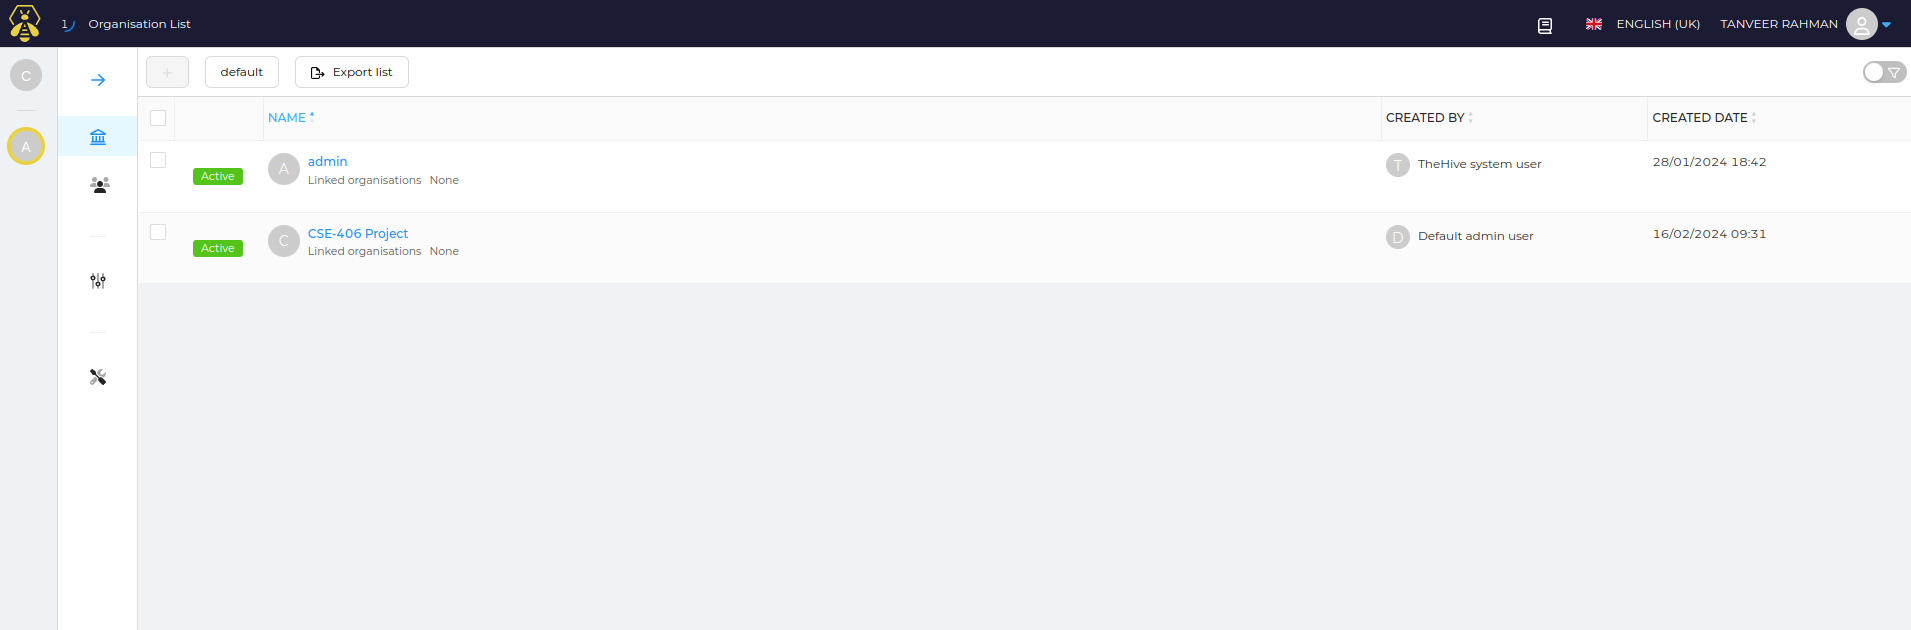
\includegraphics[width=.8\linewidth]{Case_images/Case Demo/Organizations.png}
    \caption{Newly created CSE-406 organization}
    \label{fig:organization}
\end{figure}
\bigskip
\bigskip
\begin{figure}[h]
    \centering
    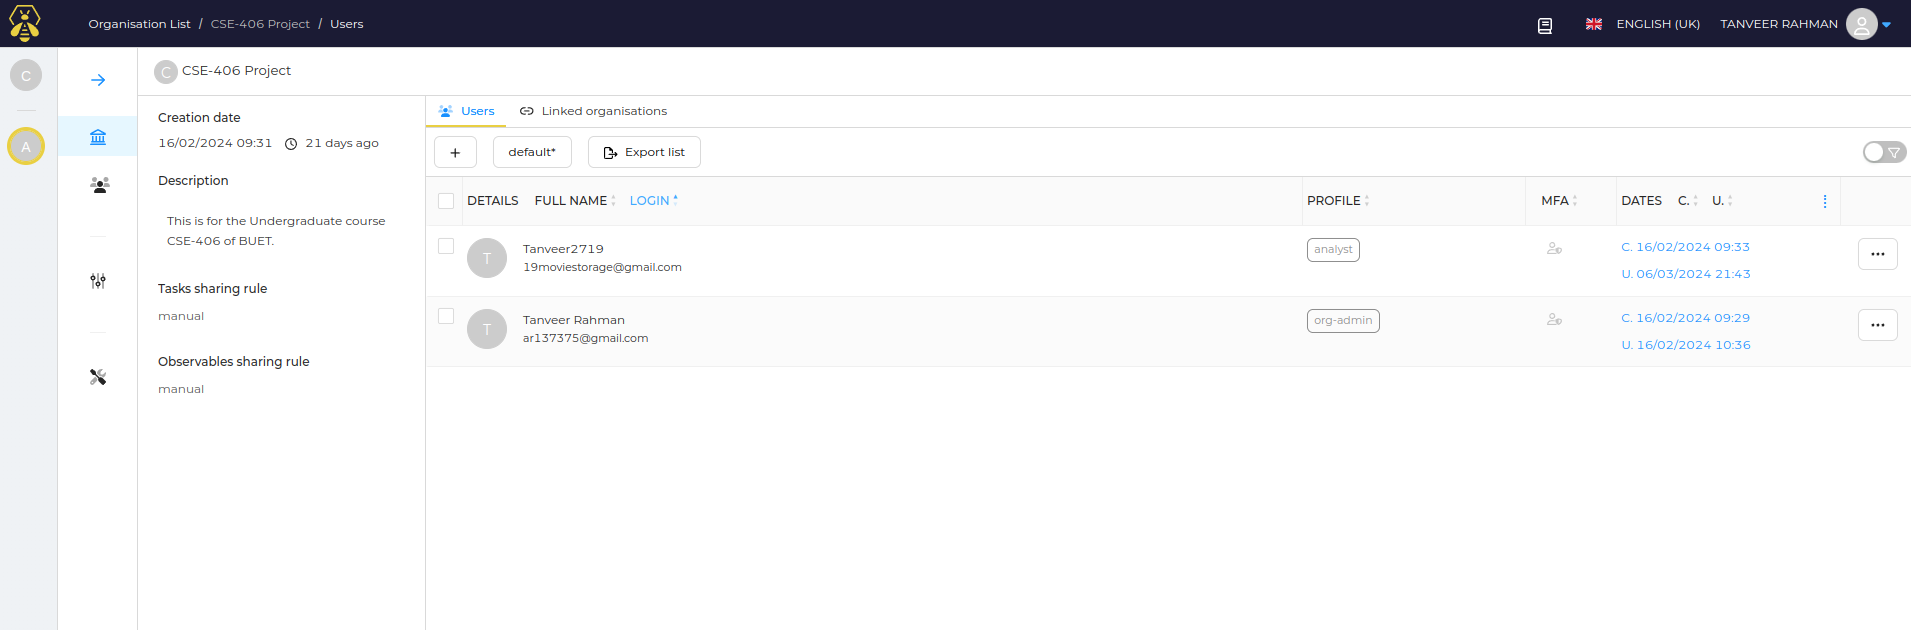
\includegraphics[width=.8\linewidth]{Case_images/Case Demo/users.png}
    \caption{Users of CSE-406}
    \label{fig:users_of_organization}
\end{figure}
\bigskip
\bigskip

\subsection{Case Creation Page}
\begin{figure}[h]
    \centering
    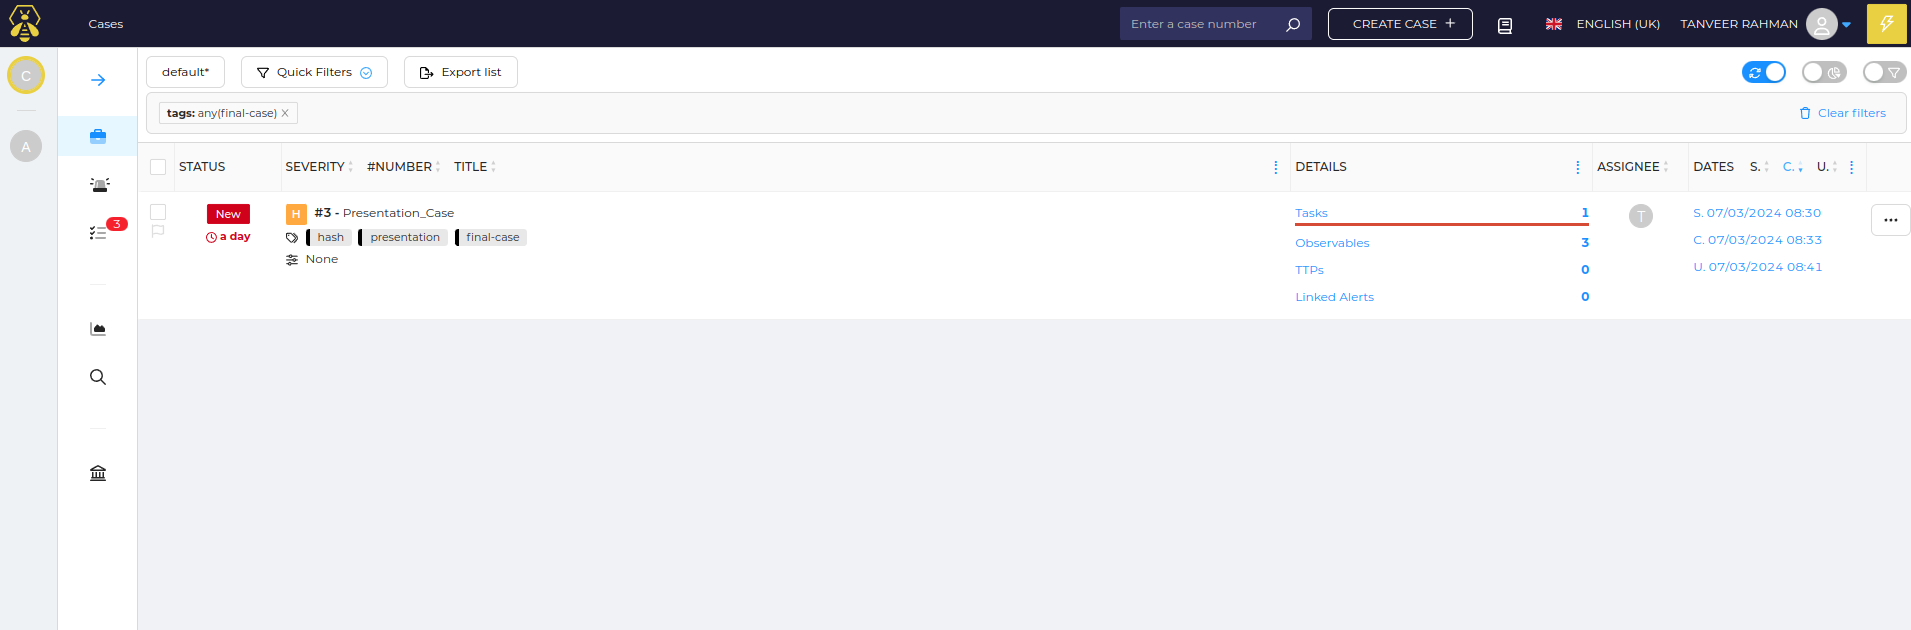
\includegraphics[width=.8\linewidth]{Case_images/Case Demo/CaseCreationpage.png}
    \caption{Cases of CSE-406}
    \label{fig:cases_of_organization}
\end{figure}
\newpage

\begin{figure}[h]
    \centering
    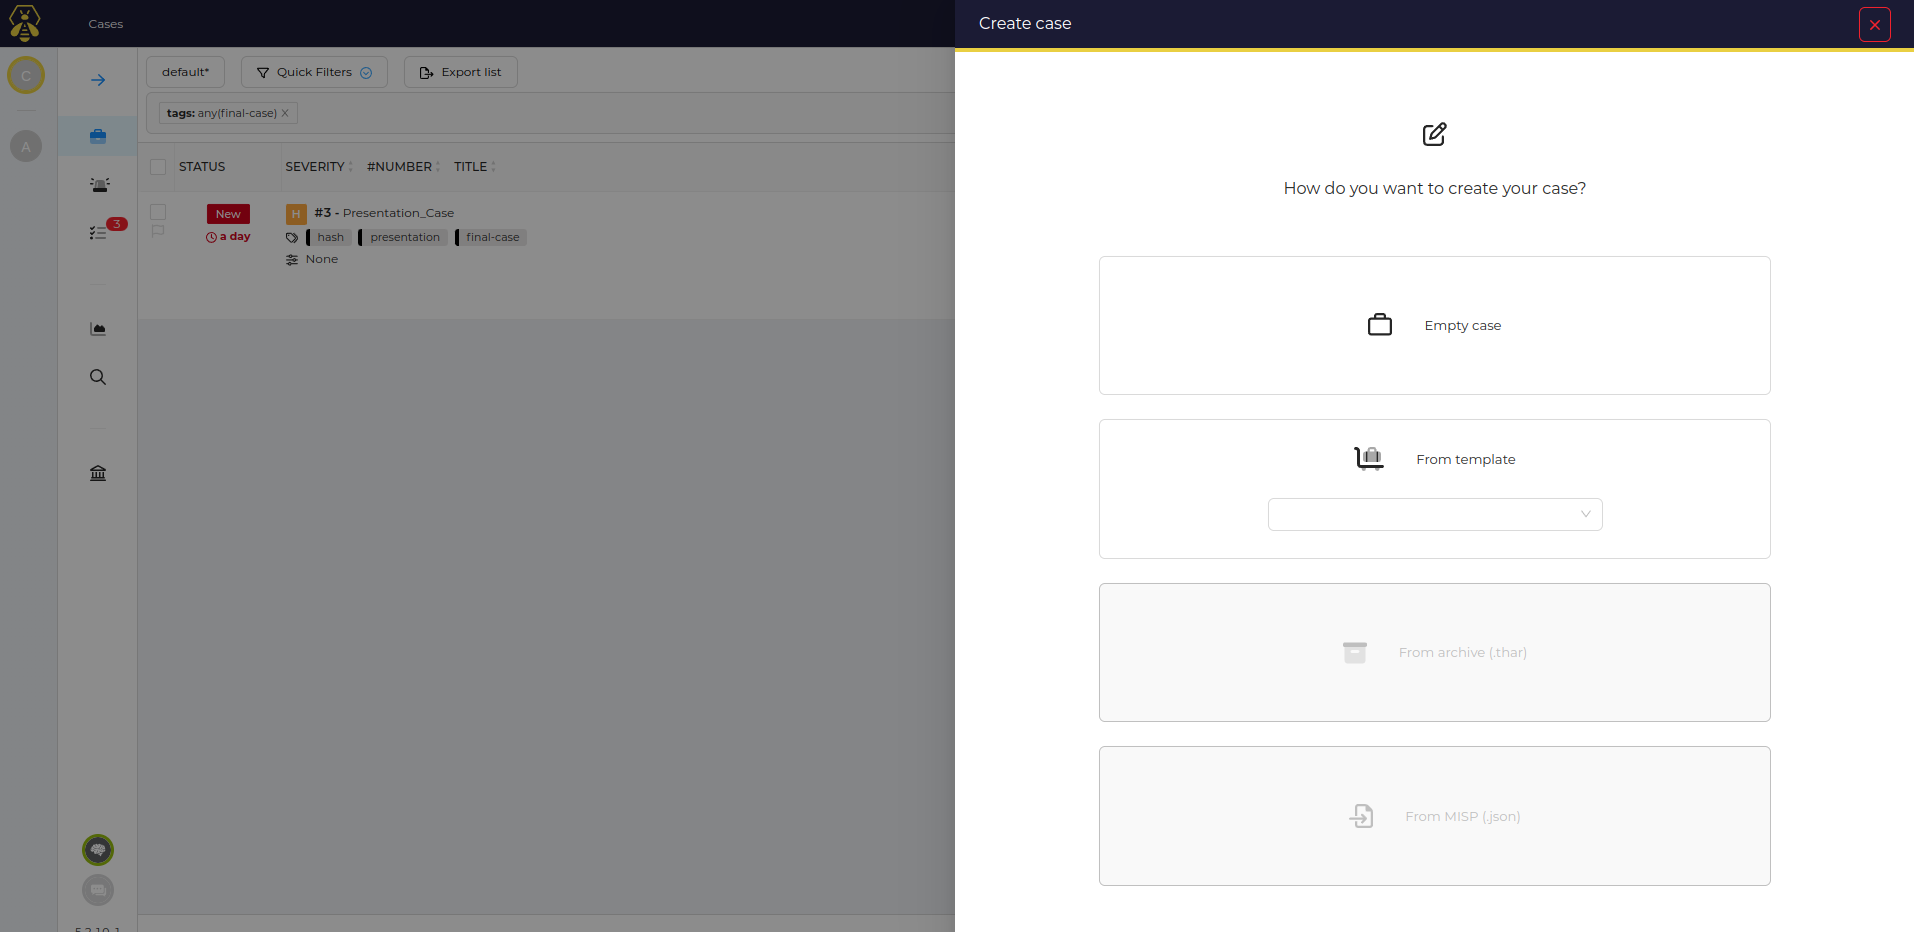
\includegraphics[width=.8\linewidth]{Case_images/Case Demo/CreateCase.png}
    \caption{Create case }
    \label{fig:create_case}
\end{figure}
\bigskip
\bigskip
\begin{figure}[h]
    \centering
    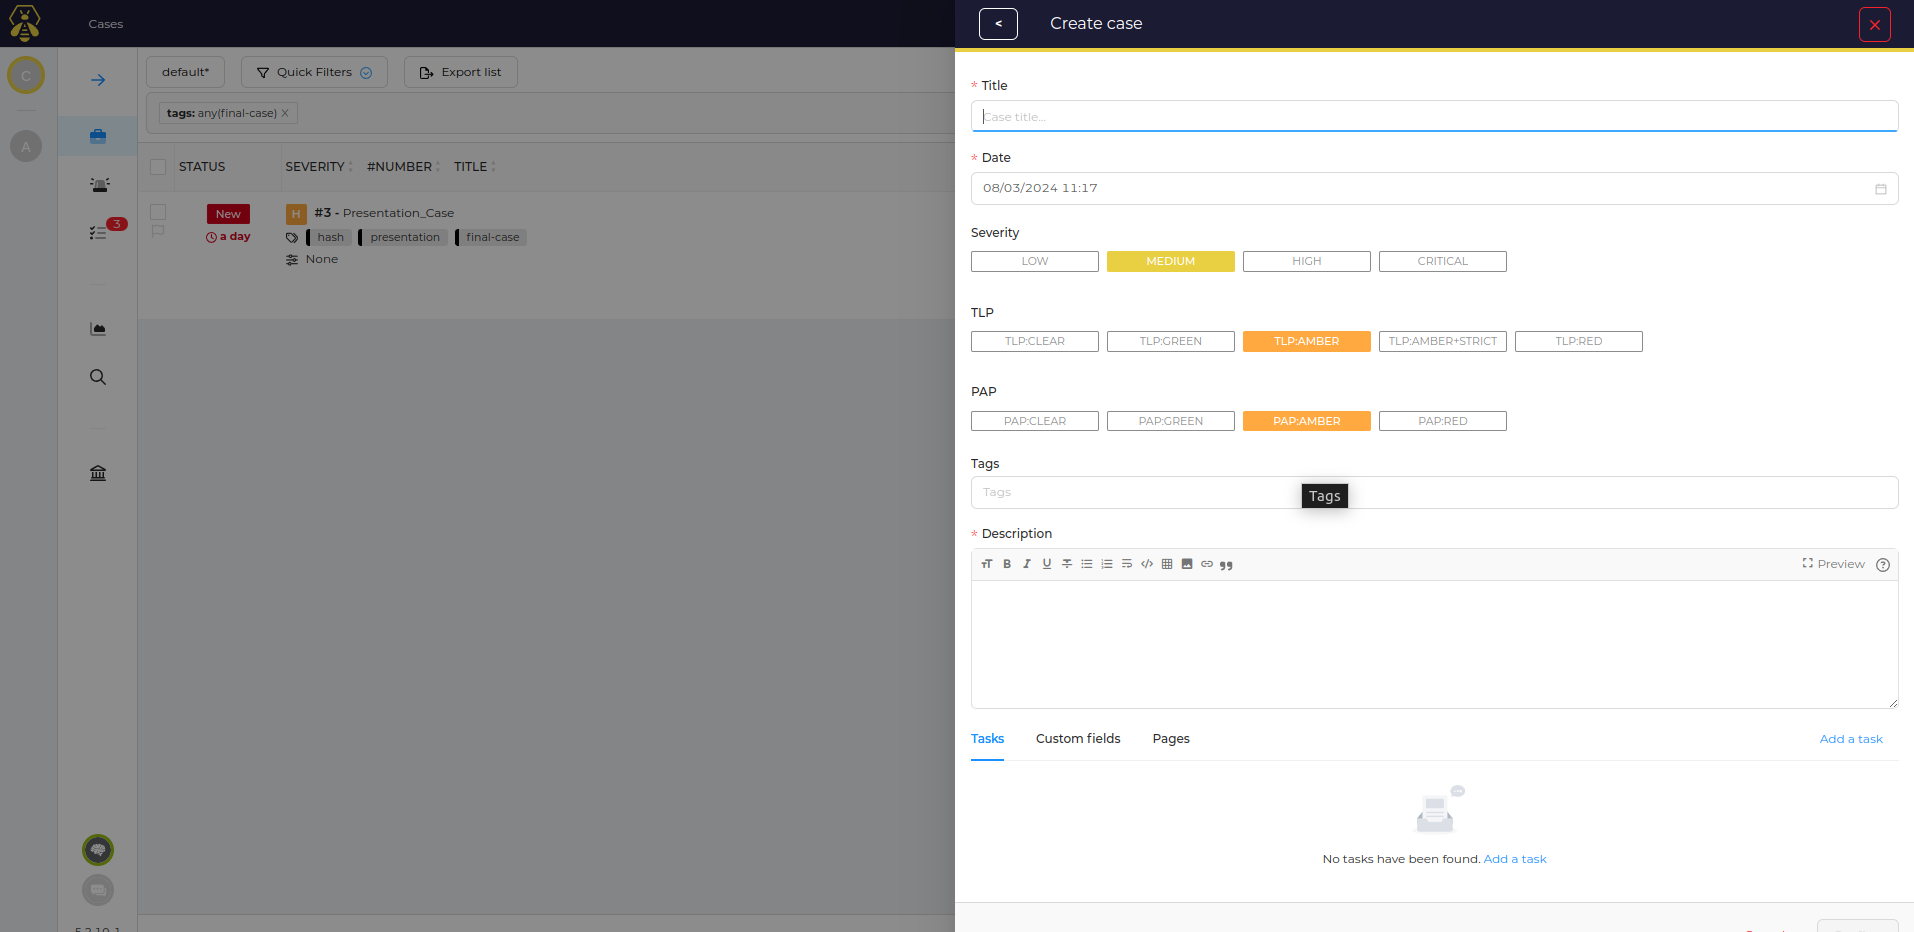
\includegraphics[width=.8\linewidth]{Case_images/Case Demo/empty_case.png}
    \caption{Empty case }
    \label{fig:empty_case}
\end{figure}
\newpage

\begin{figure}[h]
    \centering
    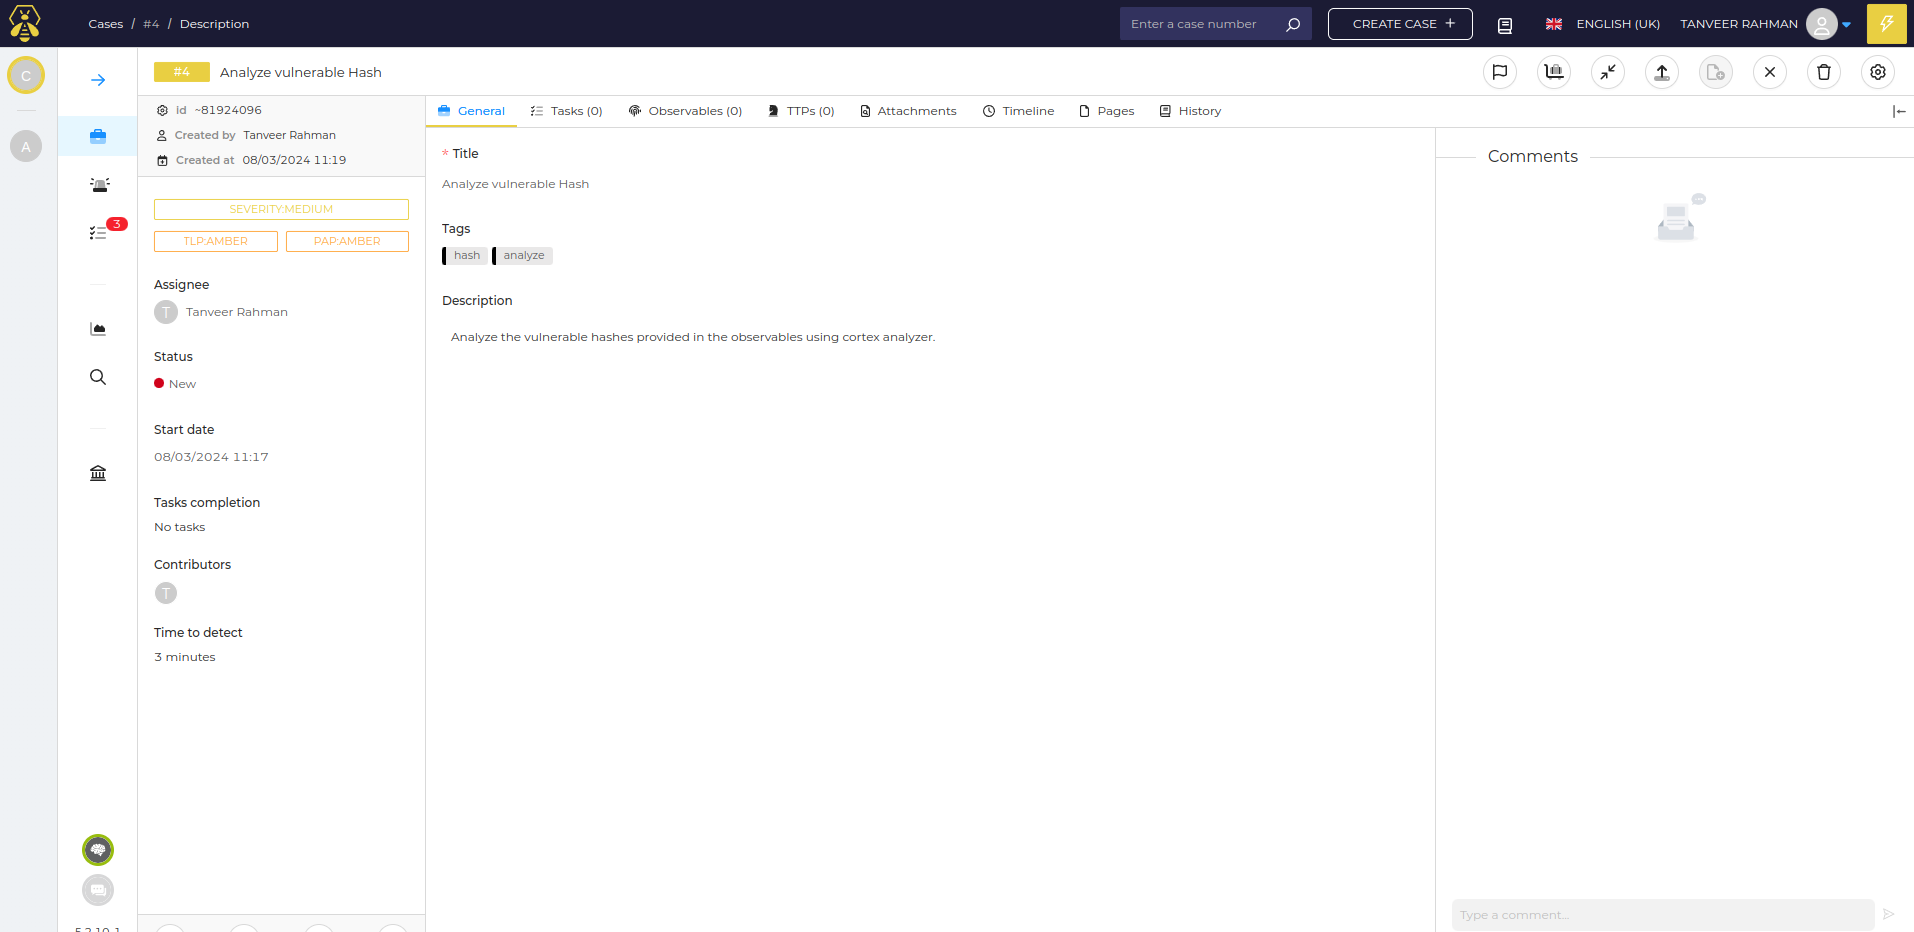
\includegraphics[width=.7\linewidth]{Case_images/Case Demo/newly_created_case.png}
    \caption{Newly Created case }
    \label{fig:newly_created_case}
\end{figure}

\subsection{Tasks}
\begin{figure}[h]
    \centering
    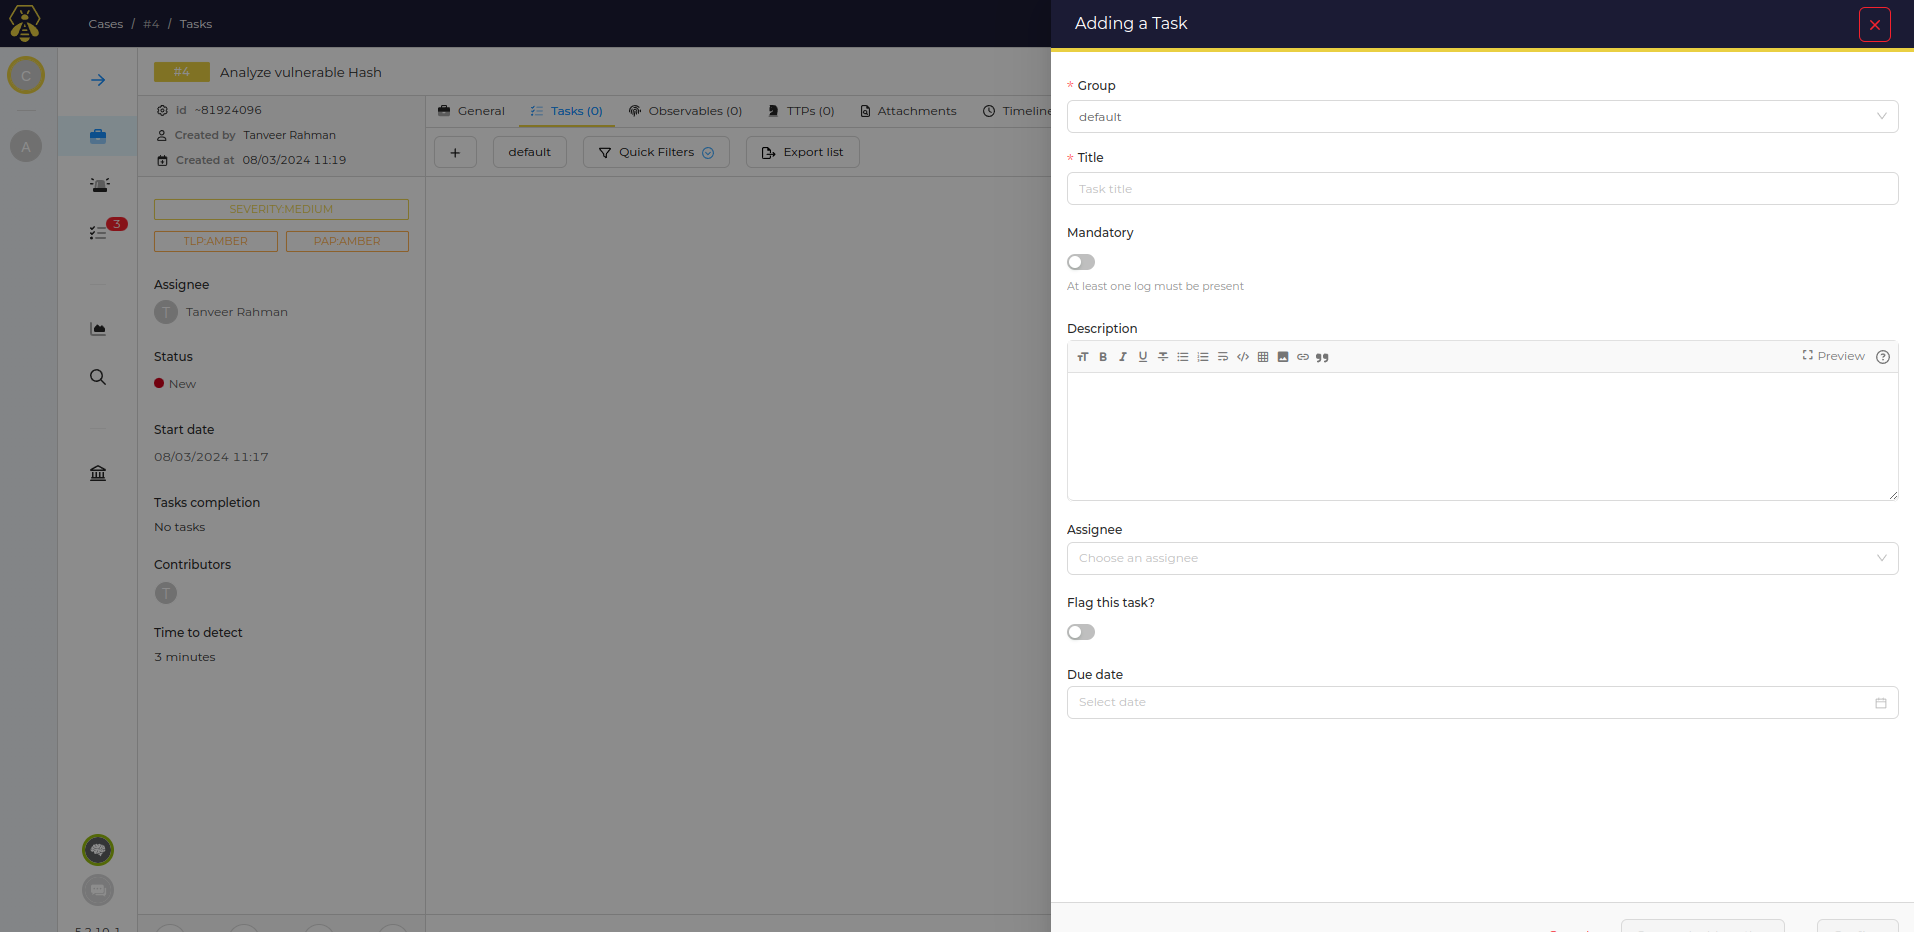
\includegraphics[width=.7\linewidth]{Case_images/Case Demo/Add_task.png}
    \caption{Add Task to the case }
    \label{fig:add_task}
\end{figure}

\begin{figure}[h]
    \centering
    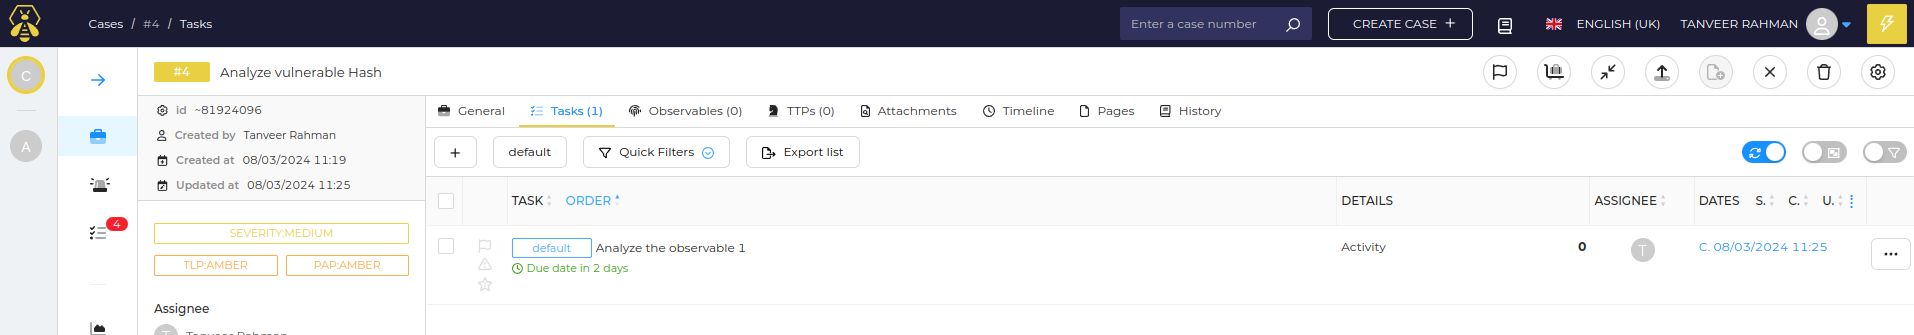
\includegraphics[width=.7\linewidth]{Case_images/Case Demo/Task_page.png}
    \caption{Tasks of the case }
    \label{fig:task_page}
\end{figure}
\newpage
\subsection{Observable}
\begin{figure}[h]
    \centering
    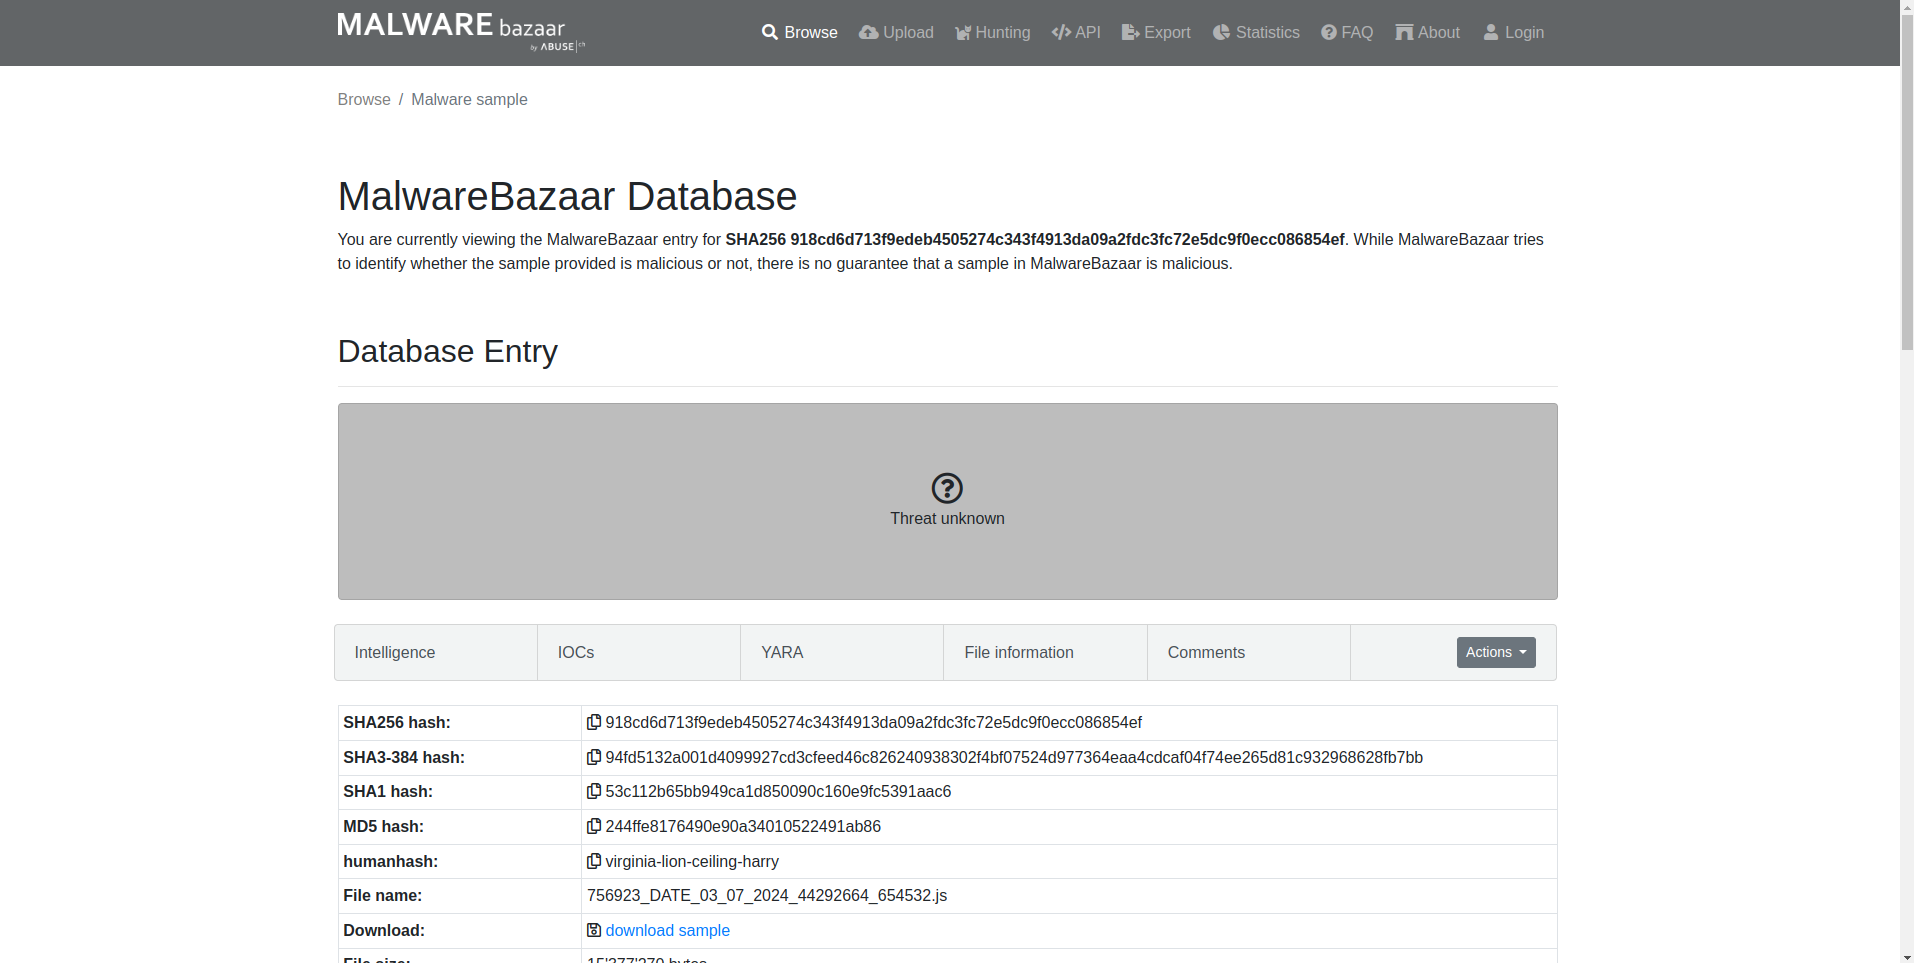
\includegraphics[width=.7\linewidth]{Case_images/Case Demo/Malwarebazar.png}
    \caption{Get Hash from MalwareBazar}
    \label{fig:hash}
\end{figure}

\begin{figure}[h]
    \centering
    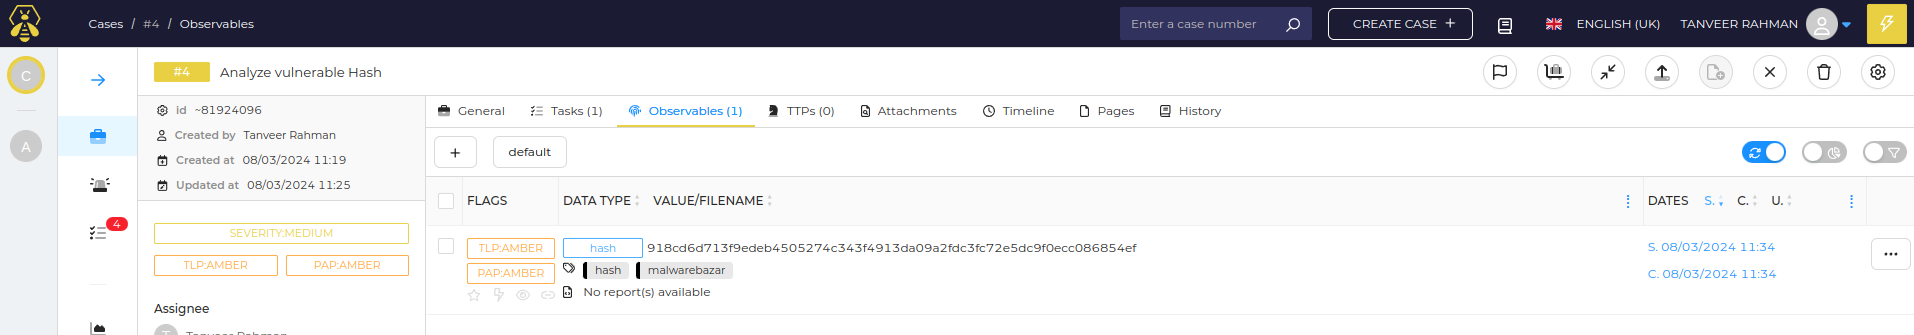
\includegraphics[width=.6\linewidth]{Case_images/Case Demo/observables.png}
    \caption{Observables List}
    \label{fig:observable_list}
\end{figure}

\begin{figure}[h]
    \centering
    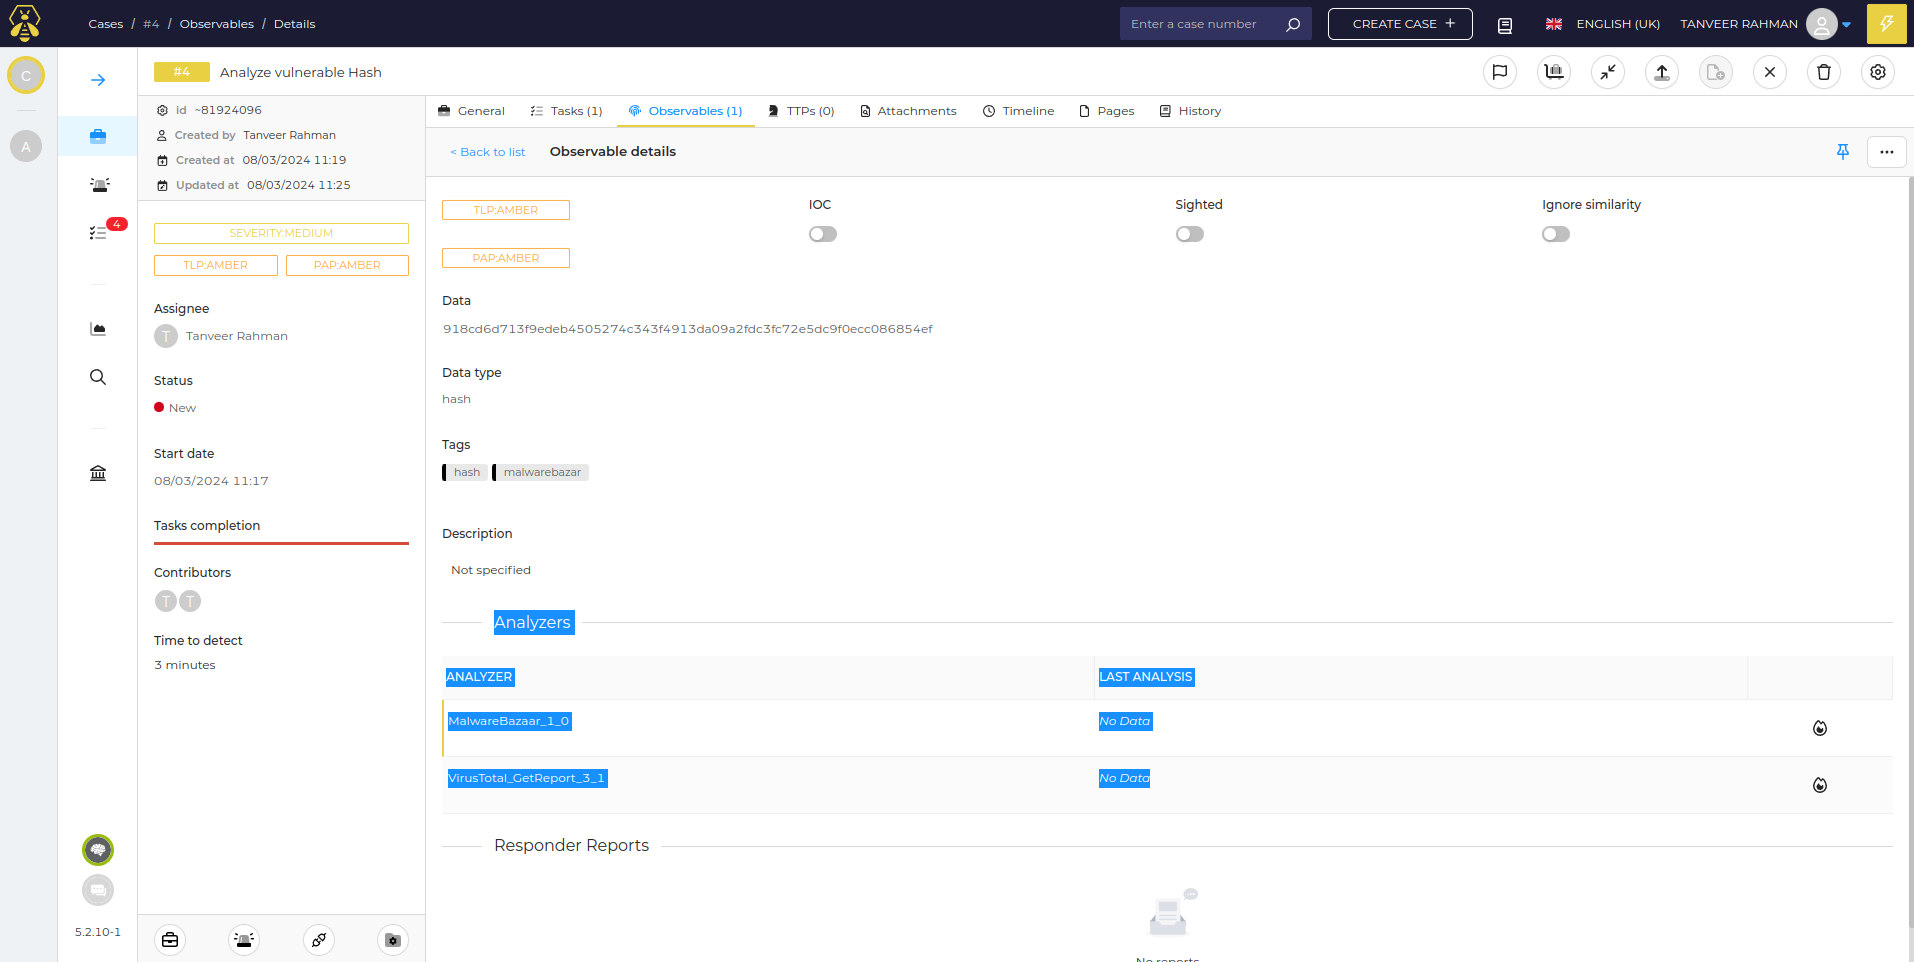
\includegraphics[width=.7\linewidth]{Case_images/Case Demo/analyze_observable.png}
    \caption{Analyze Observable}
    \label{fig:analyze_observable}
\end{figure}

\newpage
\subsection{Analyzer Reports}
\begin{figure}[h]
    \centering
    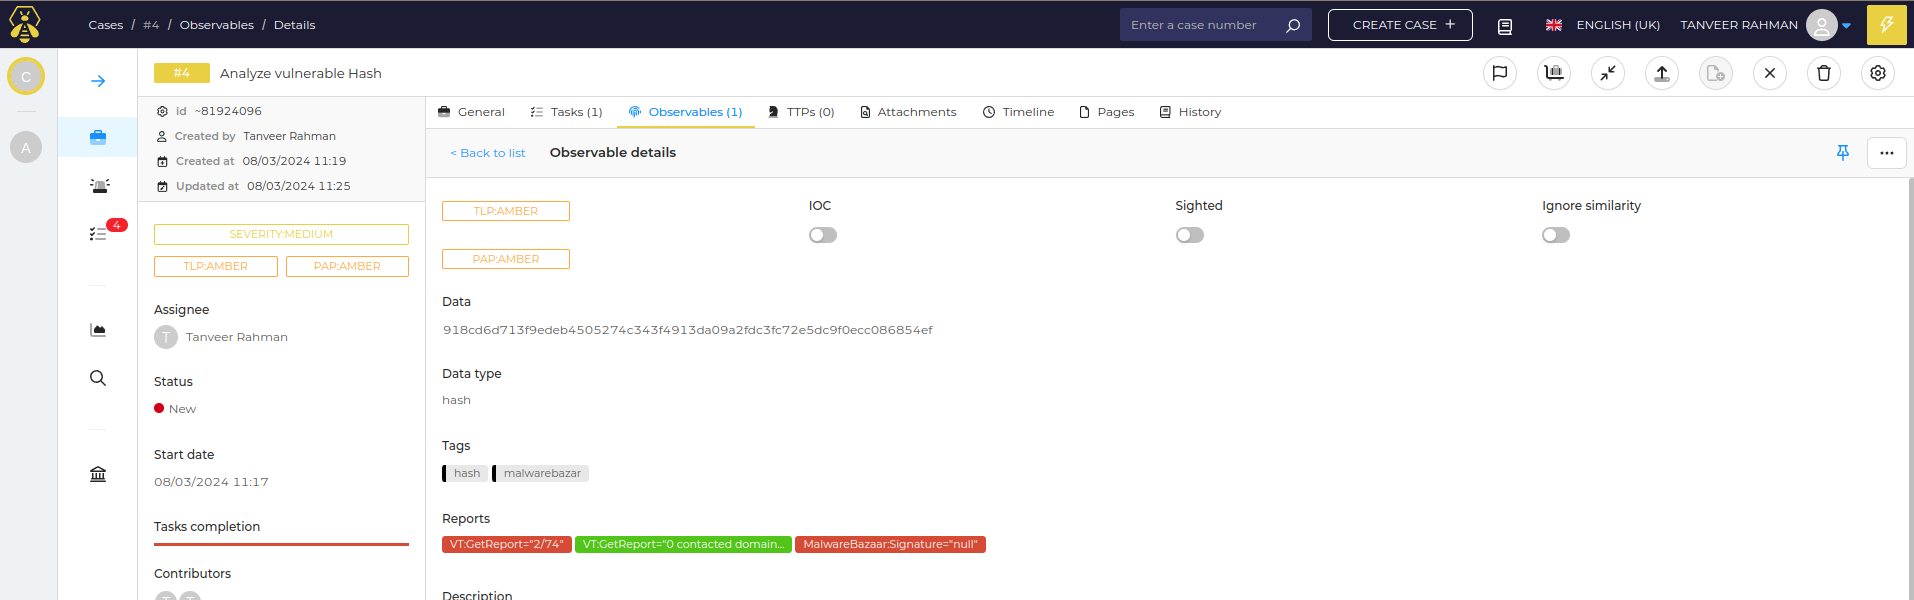
\includegraphics[width=.8\linewidth]{Case_images/Case Demo/analyzer reports.png}
    \caption{Analyzer Reports}
    \label{fig:analyzer_reports}
\end{figure}
\bigskip
After clicking the report we want to view, we get the report generated by the analyzer.
\begin{figure}[h]
    \centering
    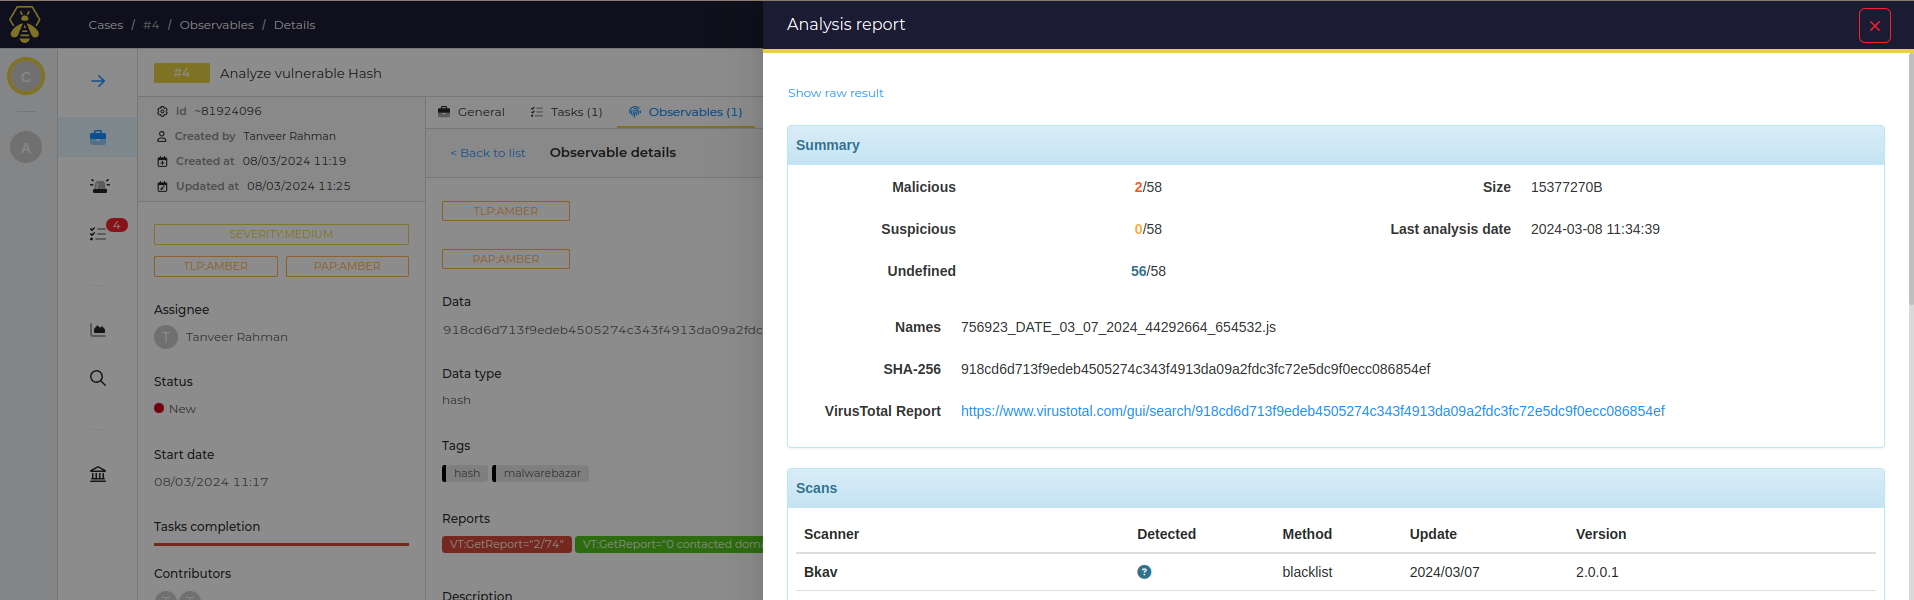
\includegraphics[width=.8\linewidth]{Case_images/Case Demo/view_report.png}
    \caption{View Report}
    \label{fig:veiw_report}
\end{figure}


    


% MOHAIMIN
\chapter{Cortex}
Cortex is a software project that complements and extends the capabilities of
TheHive, a security incident response platform. It serves as an automation
and orchestration engine. It automates the execution of various analysis
tasks and security operations related to incident response by making api
calls to various threat intelligence feeds and collects their outputs.

\section{Cortex: Key Features}

\subsection{Automation}
Cortex allows users to define and execute a wide range
of actions, such as analyzing observables, querying threat intelligence
feeds such as VirusTotal, CyberCrime-Tracker etc. and interacting with
other security tools and services.

\subsection{Analyzer Integration}
Cortex includes a collection of analyzers, which
are plugins, enabled by adding API key, can be used to analyze different types of observables, for example, IP addresses, urls, hashes etc.
These analyzers can be integrated into TheHive through Cortex and
automatically perform tasks like malware analysis, DNS lookups etc.
The generated reports can be shared with other security analysts of
the organization which saves analysts time and standardize the investigation process.

\subsection{Responder Integration}
Responders are plugins that can take action
based on the analysis results. For example, if an analyzer detects a
malicious URL, a responder can be configured to block the URL at the
firewall or update an indicator of compromise blacklist.

\subsection{Extensibility}
Cortex allows organizations to develop custom analyzers
and responders tailored to their specific needs. This flexibility makes it
a valuable tool for organizations with unique security requirements.

\subsection{Integration with TheHive}
By integrating cortex with TheHive, it
is easy to automate analysis and response actions into TheHive’s case
management and incident tracking workflows.

\newpage

\section{Cortex Analyzers}

\begin{figure}[htbp]
    \centering
    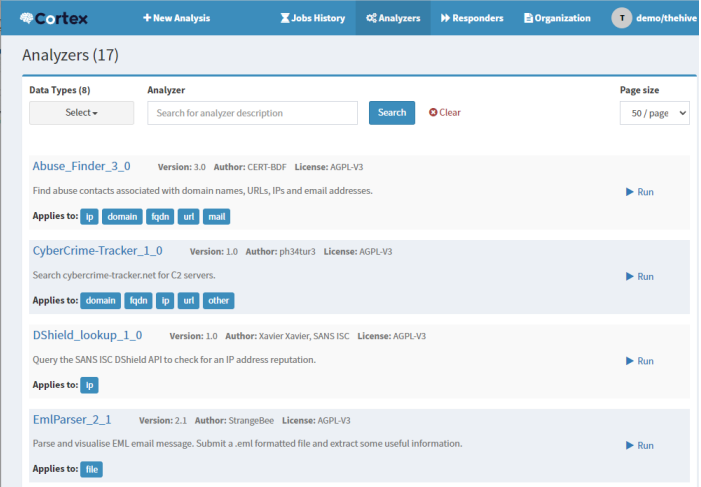
\includegraphics[width=1\linewidth]{cortex_images/cortex___1.png}
    \caption{Cortex Analyzers}
    \label{fig:Cortex Analyzers}
\end{figure}

We have used total of 216 analyzers available and
16 of them are enabled with API key. To enable a new Analyzer, we just
need to add the API key for that. A snapshot of some of the Analyzers from
Cortex is shown below.

\newpage

\section{Enabling An Analyzer}
In the Organization tab of Cortex, all the available analyzers are
provided. To enable an analyzer, press the enable button.
\begin{figure}[htbp]
    \centering
    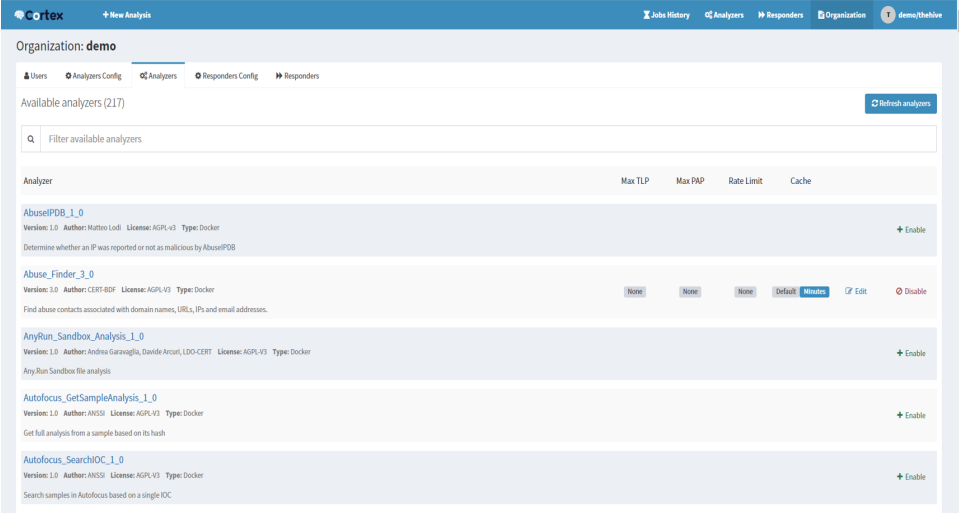
\includegraphics[width=1\linewidth]{cortex_images/cortex___2.png}
    \caption{Enabling An Analyzer}
    \label{fig:Enabling An Analyzer}
\end{figure}

The following box will be shown after pressing the enable button. To enable
an analyzer, go to it’s website and get the API key and put it here in the
key option.

\begin{figure}[htbp]
    \centering
    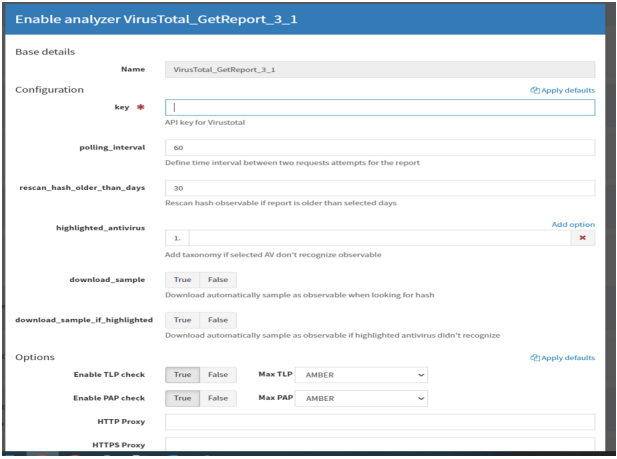
\includegraphics[width=1\linewidth]{cortex_images/image.png}
    \caption{Ading the API Key}
    \label{fig:Ading the API Key}
\end{figure}

\newpage

\section{Running An Analyzer in Cortex}
To run an analyzer, fill up the TLP, PAP, Data Type and Data and select
the suitable analyzer accordingly. We can also select multiple analyzers for
the same data.

\begin{figure}[htbp]
    \centering
    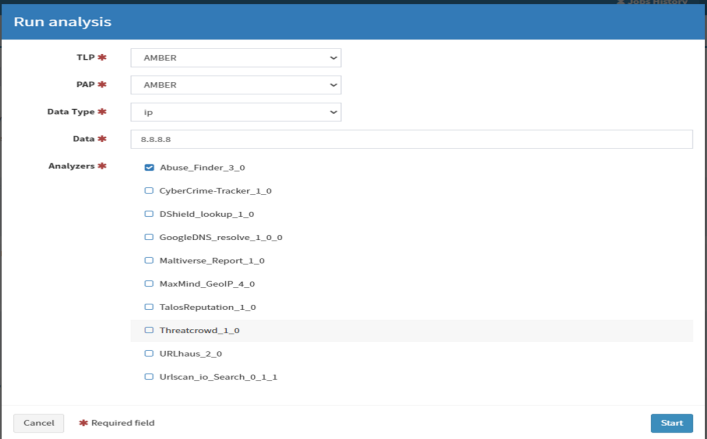
\includegraphics[width=1\linewidth]{image.png}
    \caption{Running An Analyzer}
    \label{fig:Running An Analyzer}
\end{figure}

The running log can be seen from the Jobs History in Cortex. If the status
is Success, then it has successfully generated report by querying into that
analyzer. If the status is Failure, then there may be a problem in data type
or format or the server may be down.

\begin{figure}[htbp]
    \centering
    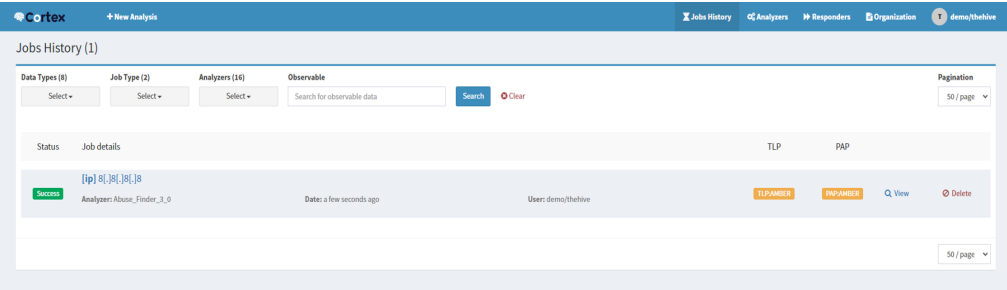
\includegraphics[width=1\linewidth]{cortex_images/12.png}
    \caption{Jobs History}
    \label{fig:enter-label}
\end{figure}

\newpage

\section{Raw Report of Analyzer}
By default in Cortex, the report generated by any analyzer is in JSON format
which is not so human readable.

\begin{figure}[htbp]
    \centering
    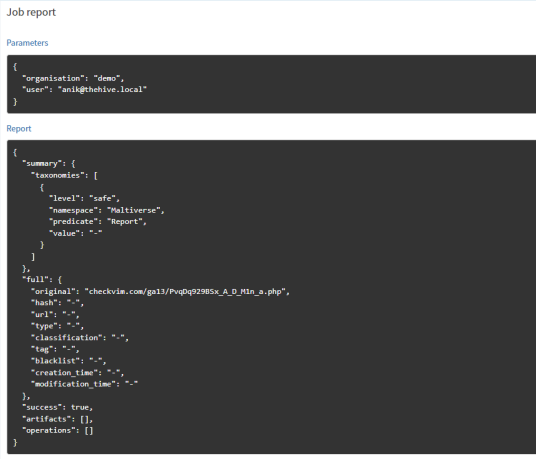
\includegraphics[width=1\linewidth]{cortex_images/13.png}
    \caption{Raw Report of Analyzer}
    \label{fig:enter-label}
\end{figure}









\chapter {Platform Integration}
\section{Integration with Cortex}
\begin{itemize}
    \item Click on Platform Management
    \item Go to Cortex
    \item Click on + in the Servers field
\end{itemize}

\begin{figure}[h]
    \centering
    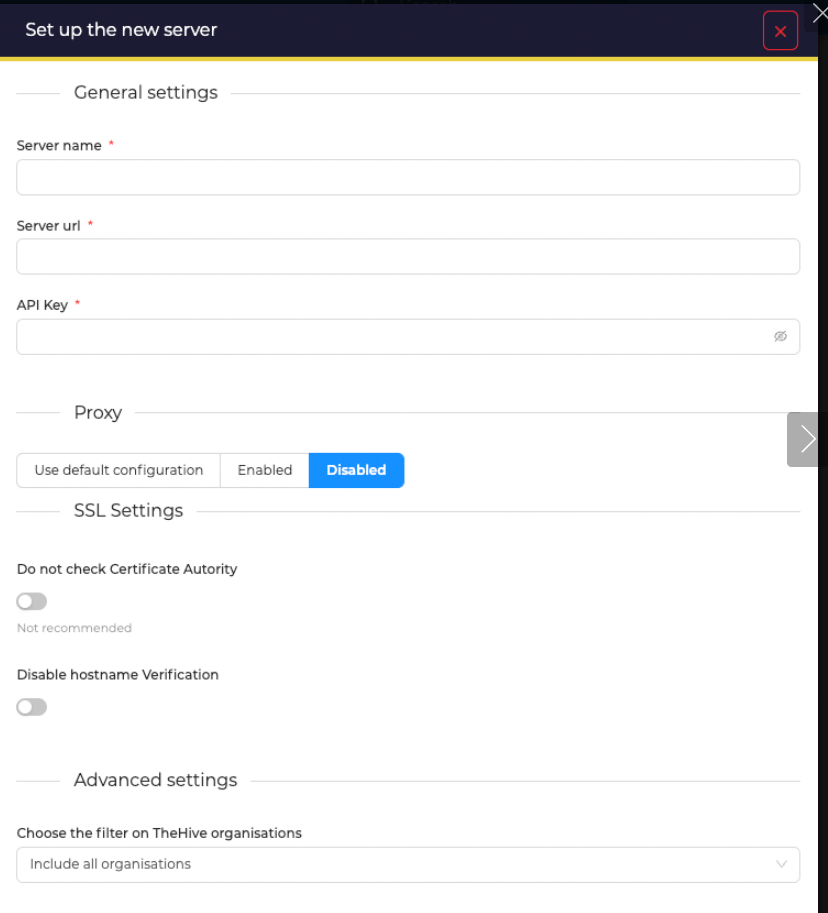
\includegraphics[width=0.6\linewidth]{Integrations Images/cortex setup.png}
    \caption{Add Cortex Server}
    \label{fig:addcortex}
\end{figure}

\newpage

\section{Integration with MISP}
One or more MISP instances can be connected to TheHive. MISP events can be imported as Alerts in TheHive. A set of filter can refine the imported events. Observables flagged as IOCs in a Case can be exported in a new event in MISP
\begin{figure}[h]
    \centering
    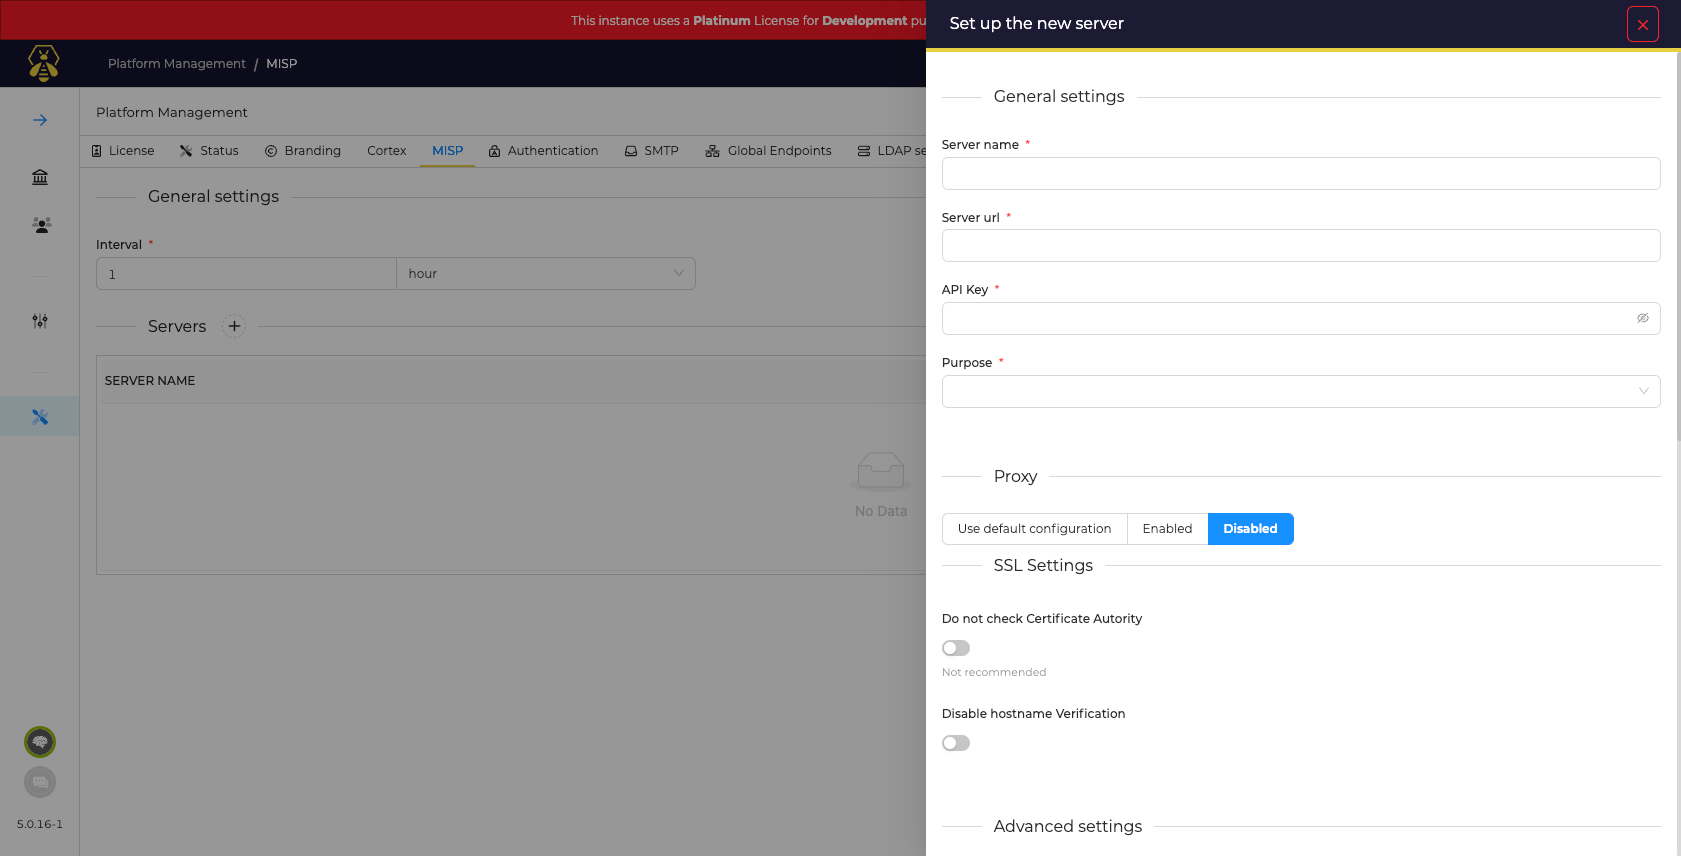
\includegraphics[width=\linewidth]{Integrations Images/platform-management-misp-1.png}
    \caption{Add Misp Server}
    \label{fig:addmisp}
\end{figure}
\newpage

\chapter{Conclusion}
The Hive is a powerful and versatile SIRS that can be used by organizations of all sizes. It is constantly being updated with new features and improvements. The platform’s automation capabilities, seamless integration with external security tools,
and comprehensive reporting and analytics empower security professionals to streamline their incident
response workflows. On the whole, as the threat landscape continues to evolve, The Hive remains a
valuable asset in enhancing an organization’s overall security posture.




\end{document}
